% ============================================================
% 03-thuc-nghiem.tex — Chương 3: thực nghiệm trên dữ liệu tín dụng thật
% Mọi con số kết quả lấy từ macro \soLieu... (results/so-lieu*.tex) hoặc bảng sinh tự động (results/bang/*.tex).
% Tên trong mã: TN1 = E5 + E7, TN2 = E3 + E6, TN3 = E8, TN4 = E9, TN5 = E10; profile cụm = E4.
% ============================================================
\chapter{THỰC NGHIỆM VÀ ĐÁNH GIÁ}
\label{chap:thuc-nghiem}

Chương này trả lời câu hỏi của tiểu luận: \emph{\cauHoiTong} Sau 2 mục về dữ liệu (mục~\ref{sec:du-lieu}) và thiết kế
thực nghiệm (mục~\ref{sec:thiet-lap}), 4 câu hỏi nghiên cứu được trả lời theo thứ tự của quy trình đề xuất
(mục~\ref{sec:de-xuat}), cũng là thứ tự nhóm thực hiện: mục~\ref{sec:diem-xuat-phat} cho CH1 (hướng ban đầu, PSO tìm tâm
khởi tạo, và lý do chuyển hướng),
mục~\ref{sec:pso-trong-so} cho CH2 (PSO tìm trọng số so với các đối chứng), mục~\ref{sec:phien-ban-trong-so} cho CH3 (5
phiên bản PSO khi tìm trọng số) và mục~\ref{sec:kiem-chung} cho CH4 (kiểm chứng trên mẫu độc lập và giới hạn). Mục~\ref{sec:dien-giai} đọc
các phân khúc để diễn giải rủi ro, và mục~\ref{sec:danh-gia-chung} đánh giá chung từng thuật toán.

% Giang
\section{Dữ liệu và tiền xử lý}
\label{sec:du-lieu}

Bài toán là phân nhóm khách hàng vay thành $c$ cụm mờ bằng FCM, chỉ dựa trên thuộc tính tài chính và lịch sử trả nợ,
sao cho các cụm khác nhau rõ về mức rủi ro. Không thuật toán nào nhìn thấy nhãn vỡ nợ; nhãn chỉ dùng để đánh giá phân hoạch
(chênh tỉ lệ vỡ nợ, AUC phân hoạch) và để lấy mẫu phân tầng bộ Taiwan. Khách hàng có độ thuộc chia đều cho nhiều cụm là
khách hàng ``biên'', loại khách hàng mà phân cụm mờ được kỳ vọng mô tả tốt hơn phân cụm cứng.

\subsection{Dữ liệu}

Bộ chính thứ nhất là dữ liệu dự báo tình trạng khó khăn tài chính của doanh nghiệp niêm yết Việt Nam \parencite{tran2022distress}: 3.277
quan sát doanh nghiệp--năm của 825 công ty trên HOSE, HNX và UPCOM giai đoạn 2010--2020, trừ ngành tài chính, ngân hàng
và bảo hiểm, mỗi quan sát có 25 chỉ số tài chính X1--X25 (thanh khoản, đòn bẩy, rủi ro kinh doanh, thị trường, định
giá). Nhãn bằng 1 khi công ty thuộc nhóm gặp khó khăn tài chính (vốn chủ sở hữu âm, hoặc EBITDA nhỏ hơn lãi vay 2 năm liên tiếp,
hoặc lợi nhuận hoạt động âm 3 năm liên tiếp), chiếm \soLieuMoTaVietNamNhanMot\% số quan sát; nhãn gán theo công ty
chứ không theo từng năm. Đây là rủi ro tín dụng doanh nghiệp, tức khả năng trả nợ của công ty đi vay.

Bộ chính thứ hai là Default of Credit Card Clients của Đài Loan \parencite{yeh2009default,uciTaiwanDefault2009}: 30.000
chủ thẻ năm 2005, 23 thuộc tính gồm hạn mức, nhân khẩu học, tình trạng trả nợ 6 tháng (PAY\_0, PAY\_2--PAY\_6), dư nợ
sao kê và số tiền đã trả; nhãn bằng 1 khi khách hàng vỡ nợ ở tháng kế tiếp (\soLieuMoTaTaiwanKiemChungNhanMot\%). Nhóm
lấy 2 mẫu con phân tầng theo nhãn, mỗi mẫu 5.000 khách hàng, không giao nhau. ``Taiwan Default'' trong chương luôn chỉ mẫu
kiểm chứng; mẫu thiết kế đã dùng trong các thí nghiệm thử và được dùng lại ở TN5 làm mẫu độc lập để kiểm trọng số. Với bộ
Việt Nam, TN5 chia các quan sát thành 2 nửa theo mã doanh nghiệp (mọi năm của một công ty nằm cùng một nửa), chuẩn hoá
riêng từng nửa (\texttt{viet\_nam\_nua}). Bộ Việt Nam đã được dùng khi thiết kế, nên một phát hiện chỉ được coi là vững
khi lặp lại trên Taiwan Default và trên mẫu độc lập.

Bảng~\ref{tab:tu-dien-vn} và~\ref{tab:tu-dien-taiwan} liệt kê thuộc tính của 2 bộ chính; các tên cột này được dùng
trong phần kết quả và diễn giải.

\begin{table}[htbp]
\centering
\caption{Thuộc tính của bộ dữ liệu Việt Nam (theo Phụ lục A của~\cite{tran2022distress})}
\label{tab:tu-dien-vn}
\footnotesize
\setlength{\tabcolsep}{4pt}
\renewcommand{\arraystretch}{1.12}
\begin{tabular}{@{}>{\raggedright\arraybackslash}p{2.7cm}>{\raggedright\arraybackslash}p{8.9cm}>{\raggedright\arraybackslash}p{3.2cm}@{}}
\toprule
Cột & Ý nghĩa & Nhóm \\
\midrule
X1, X2, X3$^{*}$ & Tỉ số tiền mặt; tỉ số thanh toán nhanh; tỉ số thanh toán hiện hành & Thanh khoản \\
X4, X5 & Nợ dài hạn / vốn chủ sở hữu (VCSH); nợ dài hạn / tổng tài sản & Tài chính (đòn bẩy) \\
X6, X7 & Tổng nợ / VCSH; tổng nợ / tổng tài sản & Tài chính (đòn bẩy) \\
X8, X9 & Nợ ngắn hạn / VCSH; nợ ngắn hạn / tổng tài sản & Tài chính (đòn bẩy) \\
X10, X11 & Phải trả người bán / VCSH; phải trả người bán / tổng tài sản & Kinh doanh \\
X12 & Tổng tài sản / tổng nợ & Kinh doanh \\
X13 & EBITDA / (nợ ngắn hạn + lãi vay) & Kinh doanh \\
X14, X15$^{*}$ & P/E; P/E pha loãng & Thị trường \\
X16, X17, X18$^{*}$ & P/B; P/S (giá / doanh thu); giá / giá trị sổ sách hữu hình & Thị trường \\
X19 & Vốn hoá thị trường & Thị trường \\
X20 & Giá / dòng tiền (P/CF) & Thị trường \\
X21$^{*}$, X22 & Giá trị doanh nghiệp (EV); EV / doanh thu & Định giá \\
X23, X24 & EV / EBITDA; EV / EBIT & Định giá \\
X25 & Lợi nhuận trên mỗi cổ phiếu pha loãng (EPS) & Định giá \\
\addlinespace
Financial\_Distress & Nhãn: 1 nếu công ty thuộc nhóm gặp khó khăn tài chính, 0 nếu không; chỉ dùng để đánh giá & Nhãn \\
\bottomrule
\end{tabular}
\par\smallskip\parbox{\linewidth}{\scriptsize $^{*}$ Cột bị loại vì gần trùng với cột khác (mục~\ref{sec:tien-xu-ly}); còn 21
thuộc tính. Các cột định danh (mã công ty, tên, sàn, năm) không đưa vào phân cụm; mã công ty chỉ dùng để chia 2 nửa ở TN5.}
\end{table}

\begin{table}[htbp]
\centering
\caption{Thuộc tính của bộ dữ liệu Taiwan Default (theo mô tả của UCI~\cite{uciTaiwanDefault2009})}
\label{tab:tu-dien-taiwan}
\footnotesize
\setlength{\tabcolsep}{4pt}
\renewcommand{\arraystretch}{1.12}
\begin{tabular}{@{}>{\raggedright\arraybackslash}p{3.2cm}>{\raggedright\arraybackslash}p{9.0cm}>{\raggedright\arraybackslash}p{2.6cm}@{}}
\toprule
Cột & Ý nghĩa & Nhóm \\
\midrule
LIMIT\_BAL & Hạn mức tín dụng (Đài tệ) & Hạn mức \\
SEX, EDUCATION, MARRIAGE, AGE & Giới tính; trình độ học vấn; tình trạng hôn nhân; tuổi & Nhân khẩu học \\
PAY\_0, PAY\_2--PAY\_6 & Tình trạng trả nợ từ tháng 9 lùi về tháng 4 năm 2005: $-1$ trả đúng hạn, 1 đến 9 là trễ 1 đến 9 tháng;
dữ liệu còn các mã $-2$ và 0 không được mô tả. Giá trị dương là có trễ hạn & Lịch sử trả nợ \\
BILL\_AMT1--BILL\_AMT6 & Dư nợ sao kê từ tháng 9 lùi về tháng 4 (Đài tệ); có giá trị âm & Dư nợ \\
PAY\_AMT1--PAY\_AMT6 & Số tiền đã trả từ tháng 9 lùi về tháng 4 (Đài tệ) & Thanh toán \\
\addlinespace
default payment next month & Nhãn: 1 nếu vỡ nợ ở tháng kế tiếp, 0 nếu không; chỉ dùng để đánh giá & Nhãn \\
\bottomrule
\end{tabular}
\par\smallskip\parbox{\linewidth}{\scriptsize Cả 23 thuộc tính được giữ; cột mã khách hàng bị bỏ. Tên PAY\_0 là tháng đầu tiên,
bộ dữ liệu không có cột PAY\_1.}
\end{table}

TN2 và TN3 dùng thêm 5 bộ dữ liệu rủi ro công khai, gồm 3 bộ tín dụng cá nhân và 2 bộ phá sản doanh nghiệp (phá sản là dạng vỡ nợ nặng nhất của doanh nghiệp, nên dùng làm dữ liệu thay thế cho rủi ro tín dụng doanh nghiệp): South German Credit \parencite{gromping2019sgc}; German Credit bản số 24 cột
\parencite{uciGermanStatlog1994}; Australian Credit Approval \parencite{uciAustralian1987}; Polish Companies
Bankruptcy, năm thứ ba \parencite{uciPolish2016,zieba2016polish}; Taiwanese Bankruptcy Prediction
\parencite{uciTaiwanBankruptcy2020,liang2016bankruptcy}. Hai bộ phá sản được lấy mẫu phân tầng 5.000 quan sát.

Bảng~\ref{tab:mo-ta-du-lieu} mô tả các bộ sau tiền xử lý. Hai bộ chính có phần lớn thuộc tính số liên tục, bất đối xứng
vừa phải sau log (trung vị $|$hệ số bất đối xứng$|$ \soLieuMoTaVietNamLech{} và \soLieuMoTaTaiwanKiemChungLech) và số chiều hiệu
dụng khoảng một nửa số chiều (\soLieuMoTaVietNamDHieuDung{} trên \soLieuMoTaVietNamD{} và
\soLieuMoTaTaiwanKiemChungDHieuDung{} trên \soLieuMoTaTaiwanKiemChungD). Bản Taiwan chưa lấy log có đuôi dài hơn hẳn
(hệ số bất đối xứng \soLieuMoTaTaiwanKiemChungKhongLogLech, \soLieuMoTaTaiwanKiemChungKhongLogNgoaiLai\% điểm ngoại lai). Ba bộ tín
dụng cá nhân nhỏ, đa số thuộc tính là mã định danh hoặc thứ bậc. Hai bộ phá sản nhiều chiều (\soLieuMoTaPolishD{} và
\soLieuMoTaTaiwanPhaSanD), đuôi cực dài kể cả sau log (độ nhọn dư \soLieuMoTaPolishNhon{} và
\soLieuMoTaTaiwanPhaSanNhon) và nhãn lệch mạnh.

\begin{table}[htbp]
\centering
\caption{Hồ sơ các bộ dữ liệu sau tiền xử lý}
\label{tab:mo-ta-du-lieu}
\footnotesize
\setlength{\tabcolsep}{3pt}
\begin{tabular}{@{}lrrrrrrrrr@{}}
\toprule
Bộ dữ liệu & $n$ & $D$ & \begin{tabular}[b]{@{}c@{}}Nhãn 1\\(\%)\end{tabular} & \begin{tabular}[b]{@{}c@{}}Mất\\cân bằng\end{tabular} & \begin{tabular}[b]{@{}c@{}}Bất\\đối xứng\end{tabular} & \begin{tabular}[b]{@{}c@{}}Nhọn\\dư\end{tabular} & \begin{tabular}[b]{@{}c@{}}Ngoại lai\\(\%)\end{tabular} & \begin{tabular}[b]{@{}c@{}}Cặp\\$|r|>0{,}9$\end{tabular} & $D_{90\%}$ \\
\midrule
Việt Nam & 3.277 & 21 & 13,3 & 6,5 & 1,11 & 0,6 & 15,4 & 6 & 10 \\
Taiwan Default & 5.000 & 23 & 22,1 & 3,5 & 0,89 & 0,0 & 5,9 & 0 & 13 \\
Taiwan Default (không log) & 5.000 & 23 & 22,1 & 3,5 & 2,52 & 7,8 & 12,9 & 7 & 13 \\
South German Credit & 1.000 & 20 & 30,0 & 2,3 & 0,77 & 0,5 & 12,8 & 0 & 16 \\
German Credit (bản số) & 1.000 & 24 & 30,0 & 2,3 & 1,17 & 0,4 & 17,9 & 0 & 18 \\
Australian Credit & 690 & 14 & 55,5 & 0,8 & 1,15 & 0,5 & 15,9 & 0 & 12 \\
Polish Bankruptcy & 5.000 & 64 & 4,7 & 20,2 & 1,68 & 17,2 & 24,3 & 29 & 20 \\
Taiwan Bankruptcy & 5.000 & 94 & 3,2 & 30,0 & 6,63 & 233,9 & 26,0 & 39 & 42 \\
\bottomrule
\end{tabular}
\par\smallskip\parbox{\linewidth}{\scriptsize Ghi chú: mất cân bằng: số quan sát nhãn 0 trên số quan sát nhãn 1; bất đối xứng, nhọn dư: trung vị $|$hệ số bất đối xứng$|$ và độ nhọn dư các thuộc tính sau tiền xử lý; ngoại lai: tỉ lệ điểm có ít nhất một thuộc tính $|z|>3$; $D_{90\%}$: số thành phần chính giữ 90\% phương sai.}
\end{table}


\subsection{Tiền xử lý}
\label{sec:tien-xu-ly}

FCM dùng khoảng cách Euclid, nên mọi thuộc tính phải cùng thang đo và không để vài giá trị cực lớn chi
phối khoảng cách. Bốn bước áp dụng như nhau cho mọi phương pháp: làm sạch giá trị thiếu, bỏ thuộc tính gần trùng, nén
đuôi dài bằng log có dấu, chuẩn hoá z-score (module \texttt{tien\_xu\_ly.py}, Phụ lục~\ref{app:code}).

Với bộ Việt Nam, bước khó nhất là phát hiện giá trị thiếu bị ghi thành số 0. Tổng nợ trên vốn chủ sở hữu (X6) không thể
nhỏ hơn nợ ngắn hạn trên vốn chủ sở hữu (X8), vậy mà X6 bằng 0 trong khi X8 dương ở 1.084 dòng; X7 bằng 0 trong khi X9
dương ở 1.074 dòng; tổng tài sản trên tổng nợ (X12) bằng 0 ở 1.287 dòng, điều không thể có ở doanh nghiệp đang hoạt
động. Nếu giữ nguyên, các cụm có nguy cơ tách theo ``có số 0 hay không'' thay vì theo rủi ro. Nhóm coi số 0 ở 3 cột
này là giá trị thiếu và điền trung vị của phần khác 0; số 0 ở X4, X5 (nợ dài hạn) được giữ vì có thể là thật. Bốn thuộc
tính gần trùng bị loại: X15 (tương quan 0,999 với X14), X18 (0,96 với X16), X21 (0,95 với X19) và X3 (0,944 với X2),
còn \soLieuMoTaVietNamD{} thuộc tính. Danh sách này được nhóm chọn thủ công và bỏ sót X10 (tương quan
0,966 với X8), cột vẫn được giữ trong mọi thí nghiệm. Dữ liệu gốc có dấu hiệu đã bị cắt ở phân vị 1\% và 99\% (cực trị của các cột trùng
2 phân vị này), nên không xử lý ngoại lai thêm.

Với Taiwan Default, nhóm bỏ cột mã khách hàng, giữ 23 thuộc tính. Thuộc tính tiền tệ lệch rất mạnh, và dư nợ sao kê âm
ở 1.930 trong 30.000 dòng của bộ gốc (315 dòng trong mẫu kiểm chứng). Phép $\operatorname{sign}(x)\log(1 + |x|)$ nén
đuôi dài mà vẫn giữ dấu và giữ 0, được áp dụng cho mọi thuộc tính của 2 bộ chính. Thí nghiệm thử còn cho thấy trên
bản chưa log, với $c \ge 5$, FCM khởi tạo ngẫu nhiên dừng ở các cực tiểu khác nhau; bản không log vì thế được giữ riêng
cho phần đối chiếu (mục~\ref{sec:diem-xuat-phat}). South German, German bản số và Australian không lấy log vì đa số thuộc
tính là mã thứ bậc hoặc định danh; 2 bộ phá sản bị loại cột hằng, điền trung vị cho ô trống rồi lấy log có dấu. Mọi
bộ được chuẩn hoá z-score theo cột; bản giá trị gốc được giữ để đọc profile cụm ở mục~\ref{sec:dien-giai}.

% Giang; Hà — 3.2.3
\section{Thiết kế thực nghiệm}
\label{sec:thiet-lap}

\subsection{Các thí nghiệm}
\label{sec:cac-thi-nghiem}

Bảng~\ref{tab:ch3-thi-nghiem} liệt kê 5 thí nghiệm theo thứ tự trình bày. TN1 và TN2 là hướng ban đầu: TN1 so 5 phiên bản PSO
khi tìm tâm khởi tạo, TN2 đo số cực tiểu của $J_m$ để giải thích kết quả. TN3, TN4, TN5 là phần chính, chạy sau khi chuyển hướng: TN3 so PSO-W tìm trọng số với 3 đối
chứng trên 7 bộ, TN4 so 5 phiên bản PSO khi tìm trọng số, TN5 kiểm trọng số học được trên mẫu độc lập. Thứ tự chạy thực tế
khác thứ tự trình bày; trong mã nguồn và tệp kết quả, các thí nghiệm giữ tên theo thứ tự chạy (ghi trong ngoặc ở cột đầu;
Phụ lục~\ref{app:code}).

\begin{table}[htbp]
\centering
\caption{Các thí nghiệm của tiểu luận}
\label{tab:ch3-thi-nghiem}
\footnotesize
\setlength{\tabcolsep}{3pt}
\begin{tabular}{@{}>{\raggedright\arraybackslash}p{1.2cm}>{\raggedright\arraybackslash}p{5.2cm}>{\raggedright\arraybackslash}p{4.2cm}>{\raggedright\arraybackslash}p{1.5cm}>{\raggedright\arraybackslash}p{0.9cm}>{\raggedright\arraybackslash}p{0.9cm}@{}}
\toprule
TN (mã) & Phương pháp so sánh & Dữ liệu và cấu hình & Số lượt & Câu hỏi & Mục \\
\midrule
TN1 (E5, E7) & Năm phiên bản PSO tìm tâm, $N \in \{10, 20, 30\}$ hạt, $T \in \{20, 30, 50\}$ vòng; 3 đối chứng FCM ($U$ ngẫu
nhiên, điểm ngẫu nhiên, k-means++); quỹ đạo gbest & Hai bộ chính $c = 3$; 3 cấu hình nhiều cực tiểu & \soLieuENamSoLuot{} và
\soLieuEBaySoLuot & CH1 & \ref{sec:e5-dat-j} \\
\addlinespace
TN2 (E3, E6) & FCM từ 30 khởi tạo $U$ ngẫu nhiên và 30 khởi tạo k-means++ (E6 thêm điểm ngẫu nhiên và PSO-W); đếm số cực
tiểu quan sát được & Bảy bộ tín dụng và bản Taiwan Default chưa lấy log, $m = 2$ (E3); 2 bộ chính, $m \in \{1{,}5;\ 2\}$,
$c = 2, \dots, 8$ (E6) & 60--120 mỗi cấu hình & CH1 & \ref{sec:vi-sao} \\
\addlinespace
TN3 (E8) & PSO-W tìm trọng số (10 hạt, 500 lần tính fitness); FCM k-means++, WFCM giải tích, tìm ngẫu nhiên cùng ngân sách &
Bảy bộ tín dụng, $m = 2$, $c \in \{2, 3, 4\}$ (\soLieuETamSoCauHinh{} cấu hình) & \soLieuETamSoLuot & CH2 & \ref{sec:pso-trong-so} \\
\addlinespace
TN4 (E9) & Năm phiên bản PSO tìm trọng số ở 2 ngân sách (500, 1.000 lần tính fitness); tìm ngẫu nhiên cùng ngân sách; FCM
k-means++ & Hai bộ chính, $m = 2$, $c \in \{2, 3, 4\}$ & \soLieuEChinSoLuot & CH3 & \ref{sec:phien-ban-trong-so} \\
\addlinespace
TN5 (E10) & Trọng số học trên mẫu nguồn (PSO-W, tìm ngẫu nhiên, WFCM giải tích) áp lên mẫu đích; FCM thường và PSO-W học tại
chỗ trên mẫu đích & Taiwan Default (mẫu thiết kế $\leftrightarrow$ kiểm chứng), Việt Nam (2 nửa theo doanh nghiệp), $c \in \{2,
3, 4\}$ & \soLieuEMuoiSoLuot & CH4 & \ref{sec:kiem-chung} \\
\bottomrule
\end{tabular}
\end{table}

\subsection{Môi trường, tham số và cách chạy}

Mã nguồn viết bằng Python~3.9.4 (numpy~2.0.2, scipy~1.13.1, pandas~2.3.3, scikit-learn~1.6.1), chạy trên Intel Xeon
E-2278G 3,40~GHz, Linux, nhiều tiến trình song song (8 đến 16), mỗi tiến trình một luồng BLAS. Một \emph{tác vụ} là một bộ
(cấu hình dữ liệu, seed) chạy tuần tự mọi phương pháp; một \emph{lượt} là một phương pháp chạy với một seed trên một cấu hình.
Mỗi phương pháp nhận bộ sinh số ngẫu nhiên riêng tạo từ seed, nên mọi phương pháp tìm trọng số trong cùng tác vụ dùng chung tâm
khởi tạo k-means++ và mẫu Silhouette. Mọi thí nghiệm dùng 30 seed chung, từ 1000 đến 1029; FCM dừng khi thay đổi lớn nhất của
tâm (của ma trận độ thuộc, với khởi tạo $U$ ngẫu nhiên; Thuật toán~\ref{alg:fcm}) giữa 2 vòng nhỏ hơn
$\varepsilon = 10^{-5}$, trần 10.000 vòng. Không lượt nào lỗi. Đơn vị độc lập trong mọi phép so là seed ($n = 30$), không
phải lượt.

\subsection{Kiểm định và cách báo kết quả}
\label{sec:kiem-dinh}

Ở phần trọng số, mỗi phép so là một cặp (phương pháp, đối chứng) ở một cấu hình và một chỉ số, dùng kiểm định Wilcoxon hai phía
theo cặp seed~\parencite{wilcoxon1945}; trong mỗi thí nghiệm, thủ tục Holm~\parencite{holm1979} hiệu chỉnh trên toàn bộ các
phép so ($\alpha = 0{,}05$). Kết quả được báo bằng trung vị 30 seed và số cấu hình ``tốt hơn / không khác / kém hơn''. Hai chỉ
số chính (chênh tỉ lệ vỡ nợ, AUC phân hoạch) và phép so được chốt trước khi chạy TN3--TN5, sau khi các thí nghiệm thử đã
xem chúng trên 2 bộ chính; Silhouette chỉ là chỉ số phụ vì chính nó là
fitness. Ở phần tìm tâm, mỗi phiên bản cải tiến được so với PSO gốc trên độ lệch $J$ sau PSO bằng Wilcoxon, Holm trên
\soLieuENamKdSoPhep{} phép so; tỉ lệ đạt $J$ tốt nhất chỉ được báo dạng số seed $k/30$, vì ở phần này hầu hết các
phương pháp đạt cùng một nghiệm và mô tả là đủ. Khi không có phép so nào có ý nghĩa sau hiệu chỉnh, tiểu luận viết ``không
phát hiện khác biệt'', không viết phương pháp nào tốt hơn hay kém hơn. Kiểm định theo seed chỉ cho biết khác biệt có vượt dao động ngẫu nhiên
của thuật toán trên mẫu đang xét hay không; độ bất định do lấy mẫu khách hàng nằm ngoài phép đo này và chỉ được kiểm một phần ở TN5.

% Hải — 3.3.1, 3.3.3; Bình — 3.3.2
\section{PSO tìm tâm khởi tạo cho FCM}
\label{sec:diem-xuat-phat}

Mục này trình bày hướng nhóm thực hiện trước, cách ghép PSO với FCM phổ biến nhất trong tài liệu, và trả lời CH1. TN1 dùng
5 phiên bản PSO tìm tâm (Thuật toán~\ref{alg:pso-khoi-tao}) trên lưới số hạt $N \in \{10, 20, 30\}$ và số vòng
$T \in \{20, 30, 50\}$, rồi FCM chạy tới hội tụ từ gbest. Mục~\ref{sec:e5-dat-j} so các phiên bản với nhau,
mục~\ref{sec:e5-doi-chung} so với 3 cách khởi tạo không dùng PSO, mục~\ref{sec:vi-sao} giải thích kết quả bằng số cực tiểu
của $J_m$, và mục~\ref{sec:chuyen-huong} nêu nhận xét cùng lý do nhóm chuyển sang tìm trọng số. Phép đo số cực tiểu cũng là
bước 1 của quy trình đề xuất.

\subsection{So sánh 5 phiên bản theo số hạt và số vòng}
\label{sec:e5-dat-j}

Như thuật toán tối ưu, cả 4 bản cải tiến cho gbest gần cực tiểu hơn PSO gốc: có ý nghĩa sau Holm ở
\soLieuENamKdWTotHon{} trên \soLieuENamKdSoOMoiPb{} ô với PSO-W, \soLieuENamKdSTotHon{} với PSO-S, \soLieuENamKdLogTotHon{} với
PSO-LOG và \soLieuENamKdQpsoTotHon{} với QPSO, không ô nào kém hơn. Quỹ đạo gbest (Hình~\ref{fig:e7-quy-dao}) cho thấy PSO gốc,
vốn giữ trọng số quán tính cố định bằng 1 và không giảm theo vòng, chỉ cải thiện trong vài vòng đầu (trên Taiwan Default, vòng cải thiện cuối có trung vị
\soLieuEBayTaiwanKiemChungGocHatBaKhongVongNamKhongVongCuoiTv), còn PSO-W và QPSO cải thiện tới vòng cuối.
\label{sec:e5-toi-uu}

Bảng~\ref{tab:e5-lech-taiwan_kiem_chung} cho thấy cùng hiện tượng trên cả lưới. Độ lệch của PSO gốc chỉ giảm khi tăng số hạt
(từ 26,0\% với 10 hạt xuống 22,5\% với 30 hạt trên Taiwan Default) và không đổi theo số vòng; 4 bản cải tiến giảm theo cả
số hạt lẫn số vòng, tốt nhất là PSO-W và QPSO với 30 hạt, 50 vòng (9,5\% và 10,1\%). Bộ Việt Nam cho cùng xu hướng, với QPSO tốt nhất (6,1\%). Ngay ở ô
tốt nhất, gbest vẫn cao hơn $J_m$ tốt nhất khoảng 6--10\%: PSO một mình chưa tới cực tiểu, phần còn lại do FCM làm.

\begin{table}[htbp]
\centering
\caption{TN1 -- J\textsubscript{m} của gbest sau PSO lệch J\textsubscript{m} tốt nhất (\%) trên Taiwan Default, c~=~3}
\label{tab:e5-lech-taiwan_kiem_chung}
\footnotesize
\setlength{\tabcolsep}{2pt}
\begin{tabular}{@{}lrrrrrrrrr@{}}
\toprule
& \multicolumn{3}{c}{10 hạt} & \multicolumn{3}{c}{20 hạt} & \multicolumn{3}{c}{30 hạt} \\
\cmidrule(lr){2-4} \cmidrule(lr){5-7} \cmidrule(lr){8-10}
Phiên bản & T = 20 & T = 30 & T = 50 & T = 20 & T = 30 & T = 50 & T = 20 & T = 30 & T = 50 \\
\midrule
PSO gốc (1995) & \begin{tabular}[c]{@{}c@{}}26,0\\{\scriptsize[23,8; 27,8]}\end{tabular} & \begin{tabular}[c]{@{}c@{}}26,0\\{\scriptsize[23,8; 27,8]}\end{tabular} & \begin{tabular}[c]{@{}c@{}}26,0\\{\scriptsize[23,8; 27,8]}\end{tabular} & \begin{tabular}[c]{@{}c@{}}23,2\\{\scriptsize[21,0; 24,6]}\end{tabular} & \begin{tabular}[c]{@{}c@{}}23,2\\{\scriptsize[21,0; 24,6]}\end{tabular} & \begin{tabular}[c]{@{}c@{}}23,2\\{\scriptsize[20,9; 24,6]}\end{tabular} & \begin{tabular}[c]{@{}c@{}}22,5\\{\scriptsize[20,0; 23,8]}\end{tabular} & \begin{tabular}[c]{@{}c@{}}22,5\\{\scriptsize[20,0; 23,4]}\end{tabular} & \begin{tabular}[c]{@{}c@{}}22,5\\{\scriptsize[20,0; 23,4]}\end{tabular} \\
PSO-W (1998) & \begin{tabular}[c]{@{}c@{}}19,6\\{\scriptsize[17,8; 21,3]}\end{tabular} & \begin{tabular}[c]{@{}c@{}}17,6\\{\scriptsize[15,8; 18,8]}\end{tabular} & \begin{tabular}[c]{@{}c@{}}14,7\\{\scriptsize[13,3; 15,9]}\end{tabular} & \begin{tabular}[c]{@{}c@{}}15,9\\{\scriptsize[14,0; 17,0]}\end{tabular} & \begin{tabular}[c]{@{}c@{}}13,8\\{\scriptsize[12,7; 14,8]}\end{tabular} & \begin{tabular}[c]{@{}c@{}}11,3\\{\scriptsize[10,8; 12,4]}\end{tabular} & \begin{tabular}[c]{@{}c@{}}14,8\\{\scriptsize[13,7; 15,8]}\end{tabular} & \begin{tabular}[c]{@{}c@{}}13,3\\{\scriptsize[12,6; 14,4]}\end{tabular} & \begin{tabular}[c]{@{}c@{}}9,5\\{\scriptsize[8,5; 10,9]}\end{tabular} \\
PSO-S (2022) & \begin{tabular}[c]{@{}c@{}}22,4\\{\scriptsize[20,0; 24,3]}\end{tabular} & \begin{tabular}[c]{@{}c@{}}21,7\\{\scriptsize[18,8; 23,4]}\end{tabular} & \begin{tabular}[c]{@{}c@{}}20,4\\{\scriptsize[16,7; 21,6]}\end{tabular} & \begin{tabular}[c]{@{}c@{}}18,1\\{\scriptsize[17,4; 20,3]}\end{tabular} & \begin{tabular}[c]{@{}c@{}}17,7\\{\scriptsize[15,9; 19,5]}\end{tabular} & \begin{tabular}[c]{@{}c@{}}14,8\\{\scriptsize[14,0; 17,3]}\end{tabular} & \begin{tabular}[c]{@{}c@{}}18,0\\{\scriptsize[17,1; 19,5]}\end{tabular} & \begin{tabular}[c]{@{}c@{}}16,3\\{\scriptsize[14,9; 18,4]}\end{tabular} & \begin{tabular}[c]{@{}c@{}}14,6\\{\scriptsize[13,0; 15,6]}\end{tabular} \\
PSO-LOG (2022) & \begin{tabular}[c]{@{}c@{}}21,1\\{\scriptsize[18,9; 22,7]}\end{tabular} & \begin{tabular}[c]{@{}c@{}}18,5\\{\scriptsize[17,7; 20,9]}\end{tabular} & \begin{tabular}[c]{@{}c@{}}16,8\\{\scriptsize[15,2; 18,4]}\end{tabular} & \begin{tabular}[c]{@{}c@{}}17,0\\{\scriptsize[15,2; 18,6]}\end{tabular} & \begin{tabular}[c]{@{}c@{}}16,2\\{\scriptsize[14,2; 17,4]}\end{tabular} & \begin{tabular}[c]{@{}c@{}}13,8\\{\scriptsize[12,8; 14,8]}\end{tabular} & \begin{tabular}[c]{@{}c@{}}15,9\\{\scriptsize[14,2; 17,3]}\end{tabular} & \begin{tabular}[c]{@{}c@{}}15,0\\{\scriptsize[13,7; 16,2]}\end{tabular} & \begin{tabular}[c]{@{}c@{}}13,0\\{\scriptsize[11,6; 14,1]}\end{tabular} \\
QPSO (2004) & \begin{tabular}[c]{@{}c@{}}19,3\\{\scriptsize[17,8; 22,8]}\end{tabular} & \begin{tabular}[c]{@{}c@{}}18,4\\{\scriptsize[17,8; 20,7]}\end{tabular} & \begin{tabular}[c]{@{}c@{}}17,4\\{\scriptsize[16,4; 19,8]}\end{tabular} & \begin{tabular}[c]{@{}c@{}}15,9\\{\scriptsize[13,4; 17,2]}\end{tabular} & \begin{tabular}[c]{@{}c@{}}13,9\\{\scriptsize[12,7; 14,9]}\end{tabular} & \begin{tabular}[c]{@{}c@{}}11,8\\{\scriptsize[11,0; 12,8]}\end{tabular} & \begin{tabular}[c]{@{}c@{}}13,1\\{\scriptsize[11,6; 14,4]}\end{tabular} & \begin{tabular}[c]{@{}c@{}}11,8\\{\scriptsize[10,8; 12,6]}\end{tabular} & \begin{tabular}[c]{@{}c@{}}10,1\\{\scriptsize[9,5; 10,9]}\end{tabular} \\
\multicolumn{10}{@{}l}{\textit{Đối chứng FCM (điểm ngẫu nhiên), chưa chạy FCM: 63,1}} \\
\bottomrule
\end{tabular}
\par\smallskip\parbox{\linewidth}{\scriptsize Ghi chú: trung vị và [Q1; Q3] qua 30 seed mỗi ô; đo trước khi FCM chạy; càng nhỏ thì PSO tối ưu càng tốt.}
\end{table}


Thứ hạng đó không còn sau khi FCM chạy. Trên 2 bộ chính với $c = 3$, mọi phiên bản ở mọi ô của lưới đạt $J_m$ tốt nhất ở
cả 30 seed. Trên Taiwan Default chưa lấy log với $c = 6$, cấu hình có 2 cực tiểu (mục~\ref{sec:vi-sao}), tỉ lệ đạt dao động
từ 77\% tới 100\% mà không theo số hạt, số vòng hay phiên bản (Bảng~\ref{tab:e5-luoi-taiwan_kiem_chung_khong_log}); QPSO, bản
tối ưu tốt nhất ở cấu hình này, lại cùng PSO-LOG có ô thấp nhất. Tăng ngân sách hay đổi phiên bản vì vậy không làm FCM tốt hơn.

\begin{table}[htbp]
\centering
\caption{TN1 -- tỉ lệ đạt J tốt nhất (\%) theo số hạt và số vòng trên Taiwan Default (không log), c~=~6}
\label{tab:e5-luoi-taiwan_kiem_chung_khong_log}
\footnotesize
\setlength{\tabcolsep}{3pt}
\begin{tabular}{@{}lrrrrrrrrr@{}}
\toprule
& \multicolumn{3}{c}{10 hạt} & \multicolumn{3}{c}{20 hạt} & \multicolumn{3}{c}{30 hạt} \\
\cmidrule(lr){2-4} \cmidrule(lr){5-7} \cmidrule(lr){8-10}
Phiên bản & T = 20 & T = 30 & T = 50 & T = 20 & T = 30 & T = 50 & T = 20 & T = 30 & T = 50 \\
\midrule
PSO gốc (1995) & 90 & 90 & 90 & 93 & 93 & 93 & 90 & 90 & 90 \\
PSO-W (1998) & 87 & 93 & 90 & 97 & 100 & 93 & 100 & 97 & 97 \\
PSO-S (2022) & 100 & 90 & 93 & 90 & 100 & 90 & 97 & 90 & 90 \\
PSO-LOG (2022) & 87 & 87 & 90 & 100 & 97 & 90 & 97 & 77 & 93 \\
QPSO (2004) & 97 & 97 & 90 & 93 & 83 & 87 & 93 & 77 & 87 \\
\multicolumn{10}{@{}l}{\textit{Đối chứng FCM (U ngẫu nhiên): 57\%}} \\
\multicolumn{10}{@{}l}{\textit{Đối chứng FCM (điểm ngẫu nhiên): 100\%}} \\
\multicolumn{10}{@{}l}{\textit{Đối chứng FCM (k-means++): 100\%}} \\
\bottomrule
\end{tabular}
\par\smallskip\parbox{\linewidth}{\scriptsize Ghi chú: 30 seed mỗi ô; T: số vòng PSO trước khi FCM chạy tới hội tụ.}
\end{table}


\subsection{So với khởi tạo ngẫu nhiên và k-means++}
\label{sec:e5-doi-chung}

\begin{figure}[htbp]
\centering
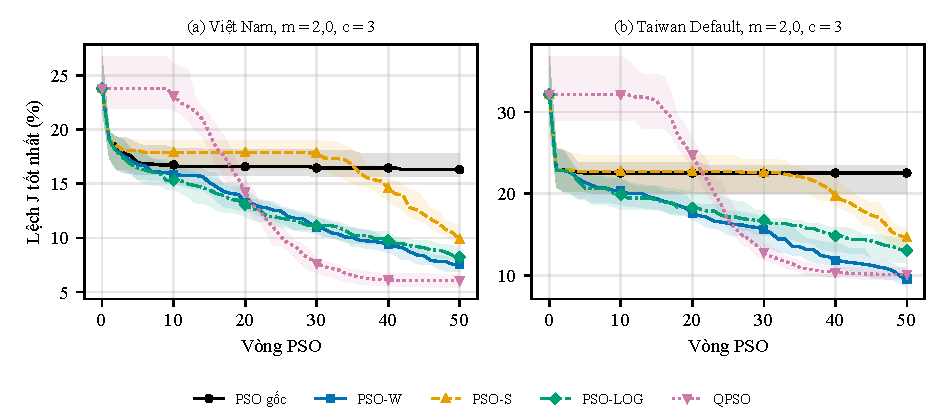
\includegraphics[width=\linewidth]{e7-quy-dao-gbest}
\caption{TN1: quỹ đạo gbest khi PSO tìm tâm (30 hạt, 50 vòng, $m = 2$, $c = 3$), đo bằng độ lệch $J_m$ của gbest so với $J_m$ tốt
nhất, theo vòng; đường là trung vị, dải màu là khoảng tứ phân vị qua 30 seed}
\label{fig:e7-quy-dao}
\end{figure}

Bảng~\ref{tab:e5-tong-hop} đặt 5 phiên bản (20 hạt, 30 vòng) cạnh 3 cách khởi tạo không dùng PSO. Trên 2 bộ chính với
$c = 3$, mọi tổ hợp PSO và mọi đối chứng,
kể cả FCM khởi tạo $U$ ngẫu nhiên, đạt $J$ tốt nhất ở mọi lượt; so theo seed với FCM k-means++, mọi lượt cho cùng $J_m$
(\soLieuENamVietNamCBaCungJKpp\% và \soLieuENamTaiwanKiemChungCBaCungJKpp\%), cùng PC và AUC, và số vòng FCM không giảm. Ở 3
cấu hình có nhiều cực tiểu, nhóm đếm số seed (trên 30) mà mỗi cách đạt cực tiểu tốt nhất. Trên Taiwan Default chưa log
($c = 6$), k-means++ đạt ở cả 30 seed (trượt \soLieuENamKhongLogDoiChungKppTruot), còn các tổ hợp PSO đạt ít hơn hoặc bằng
(tỉ lệ đạt của PSO trừ của k-means++ từ \soLieuENamKhongLogDoiChungHieuKppMin{} đến \soLieuENamKhongLogDoiChungHieuKppMax{} điểm
phần trăm). Trên Taiwan Default với $m = 1{,}5$, $c = 7$, k-means++ trượt
\soLieuEBayTaiwanKiemChungCBayDoiChungKppTruot/30 seed và mọi tổ hợp PSO đạt ít hơn k-means++
(\soLieuEBayTaiwanKiemChungCBayDoiChungHieuKppMin{} đến \soLieuEBayTaiwanKiemChungCBayDoiChungHieuKppMax{} điểm). Chỉ trên Việt
Nam với $m = 1{,}5$, $c = 8$, PSO đạt nhiều hơn k-means++ (k-means++ trượt \soLieuEBayVietNamCTamDoiChungKppTruot/30 seed, PSO
hơn \soLieuEBayVietNamCTamDoiChungHieuKppMin{} đến \soLieuEBayVietNamCTamDoiChungHieuKppMax{} điểm, tức 2--3 seed); mức chênh
này nhỏ và lấy lại được bằng cách chạy k-means++ nhiều lần (chạy lại 20 lần đạt cả 30 seed). So với FCM khởi tạo $U$ ngẫu nhiên, PSO có
tốt hơn trên Taiwan Default chưa log (FCM $U$ ngẫu nhiên chỉ đạt 57\%), đúng loại kết quả các bài báo ghi nhận; nhưng FCM khởi
tạo từ $c$ điểm dữ liệu ngẫu nhiên, tức bộ tâm của một hạt trước khi bay, đã đạt ở \soLieuENamKhongLogFcmDiemK/30 seed. Lợi
ích so với khởi tạo ngẫu nhiên vì vậy đến từ việc khởi tạo bằng tâm, không từ bước tìm kiếm của bầy. Trong khi đó PSO chậm hơn FCM k-means++ khoảng \soLieuENamTaiwanKiemChungCBaTiLeThoiGianTv{} lần trên Taiwan
Default và \soLieuENamVietNamCBaTiLeThoiGianTv{} lần trên Việt Nam (20 hạt, 30 vòng, trung vị).


\begin{table}[htbp]
\centering
\caption{TN1 -- PSO gốc và các phiên bản cải tiến làm bộ khởi tạo tâm cho FCM (20 hạt, 30 vòng, 30 seed)}
\label{tab:e5-tong-hop}
\footnotesize
\setlength{\tabcolsep}{3pt}
\begin{tabular}{@{}lrrrrrrrrr@{}}
\toprule
& \multicolumn{3}{c}{Việt Nam, c~=~3} & \multicolumn{3}{c}{Taiwan Default, c~=~3} & \multicolumn{3}{c}{Taiwan Default (không log), c~=~6} \\
\cmidrule(lr){2-4} \cmidrule(lr){5-7} \cmidrule(lr){8-10}
Phương pháp & \begin{tabular}[b]{@{}c@{}}Đạt\\(\%)\end{tabular} & \begin{tabular}[b]{@{}c@{}}Lệch\\(\%)\end{tabular} & \begin{tabular}[b]{@{}c@{}}Thời gian\\(s)\end{tabular} & \begin{tabular}[b]{@{}c@{}}Đạt\\(\%)\end{tabular} & \begin{tabular}[b]{@{}c@{}}Lệch\\(\%)\end{tabular} & \begin{tabular}[b]{@{}c@{}}Thời gian\\(s)\end{tabular} & \begin{tabular}[b]{@{}c@{}}Đạt\\(\%)\end{tabular} & \begin{tabular}[b]{@{}c@{}}Lệch\\(\%)\end{tabular} & \begin{tabular}[b]{@{}c@{}}Thời gian\\(s)\end{tabular} \\
\midrule
FCM (U ngẫu nhiên) & 100 & -- & 0,98 & 100 & -- & 0,06 & 57 & -- & 0,50 \\
FCM (điểm ngẫu nhiên) & 100 & 55,5 & 0,81 & 100 & 63,1 & 0,04 & 100 & 48,4 & 0,15 \\
FCM (k-means++) & 100 & -- & 0,88 & 100 & -- & 0,04 & 100 & -- & 0,14 \\
\midrule
PSO gốc (1995) & 100 & 17,6 & 1,65 & 100 & 23,2 & 0,97 & 93 & 21,3 & 1,61 \\
PSO-W (1998) & 100 & 10,0 & 1,48 & 100 & 13,8 & 1,30 & 100 & 17,9 & 1,85 \\
PSO-S (2022) & 100 & 13,6 & 0,94 & 100 & 17,7 & 0,80 & 100 & 20,1 & 1,64 \\
PSO-LOG (2022) & 100 & 11,8 & 1,32 & 100 & 16,2 & 0,74 & 97 & 19,1 & 1,55 \\
QPSO (2004) & 100 & 9,9 & 1,36 & 100 & 13,9 & 0,82 & 83 & 12,7 & 1,57 \\
\bottomrule
\end{tabular}
\par\smallskip\parbox{\linewidth}{\scriptsize Ghi chú: Đạt: tỉ lệ lượt đạt J tốt nhất sau khi FCM chạy tới hội tụ; lệch: J\textsubscript{m} của bộ tâm đưa vào FCM (gbest của PSO, hoặc c điểm ngẫu nhiên) so với J\textsubscript{m} tốt nhất (\%), trung vị; thời gian gồm PSO và FCM, trung vị. Bầy PSO khởi tạo bằng điểm dữ liệu ngẫu nhiên, chạy đủ số vòng, c\textsubscript{1} = c\textsubscript{2} = 2 (trừ QPSO).}
\end{table}


Các chỉ số phân cụm cũng không phân biệt được các cách khởi tạo (Bảng~\ref{tab:e5-chi-so}). Trên các lượt cho cùng nghiệm,
PC và AUC của mọi phương pháp chênh với FCM k-means++ dưới $10^{-4}$, Silhouette chênh nhiều nhất 0,018 trên 2 bộ chính.
XB thì dao động rất rộng giữa các phương pháp dù cùng nghiệm, vì 2 tâm gần trùng làm mẫu số gần bằng không
(mục~\ref{sec:chi-so}); tiểu luận vì vậy không dùng XB để so.
\label{sec:e5-chi-so}

\begin{table}[htbp]
\centering
\caption{TN1 -- chỉ số sau khi FCM hội tụ: FCM (k-means++) và mức chênh của các phương pháp còn lại}
\label{tab:e5-chi-so}
\footnotesize
\setlength{\tabcolsep}{3pt}
\begin{tabular}{@{}lrrrrrrr@{}}
\toprule
& \multicolumn{3}{c}{FCM (k-means++)} & \multicolumn{3}{c}{Chênh lớn nhất theo seed} & \\
\cmidrule(lr){2-4} \cmidrule(lr){5-7}
Cấu hình & PC & Silhouette & AUC & PC & AUC & Silhouette & XB (khoảng) \\
\midrule
Việt Nam, c = 3 & 0,373 & 0,080 & 0,840 & 8,14·10\textsuperscript{−6} & 8,88·10\textsuperscript{−6} & 0,001 & 3.677,89 -- 4.664,12 \\
Taiwan, c = 3 & 0,395 & 0,129 & 0,434 & 4,68·10\textsuperscript{−6} & 7,66·10\textsuperscript{−6} & 0,018 & 1,57·10\textsuperscript{9} -- 6,98·10\textsuperscript{9} \\
Taiwan chưa log, c = 6 & 0,196 & 0,054 & 0,545 & 3,15·10\textsuperscript{−6} & 2,74·10\textsuperscript{−5} & 0,116 & 3,33·10\textsuperscript{12} -- 3,60·10\textsuperscript{14} \\
\bottomrule
\end{tabular}
\par\smallskip\parbox{\linewidth}{\scriptsize Ghi chú: PC, Silhouette, AUC: trung vị 30 seed của FCM (k-means++); chênh lớn nhất: |hiệu| lớn nhất theo từng seed giữa một phương pháp bất kỳ (3 đối chứng, 45 tổ hợp PSO) và FCM (k-means++), chỉ trên các lượt cùng nghiệm; XB: khoảng trung vị của 8 phương pháp (3 đối chứng, 5 phiên bản PSO với 20 hạt, 30 vòng); XB không ổn định khi 2 tâm gần trùng, xem mục~\ref{sec:e5-chi-so}.}
\end{table}


\subsection{Giải thích: số cực tiểu của hàm mục tiêu}
\label{sec:vi-sao}

TN2 chạy FCM ($m = 2$) từ 30 khởi tạo độ thuộc ngẫu nhiên và 30 khởi tạo k-means++ trên mỗi bộ, mỗi $c$, rồi gom các $J_m$
cuối lệch nhau không quá $10^{-4}$ (tương đối) thành một mức; số mức là số cực tiểu \emph{quan sát được}, không phải phép chứng
minh $J_m$ chỉ có từng ấy cực tiểu. Một lượt là \emph{sụp} khi mọi tâm dồn về trung bình dữ liệu (độ lớn tâm dưới $10^{-3}$
trên dữ liệu z-score), tức mọi độ thuộc bằng $1/c$ (Bảng~\ref{tab:e3-chan-doan}).

\begin{table}[htbp]
\centering
\caption{TN2 -- chẩn đoán số cực tiểu của J\textsubscript{m}: FCM từ 30 khởi tạo mỗi kiểu}
\label{tab:e3-chan-doan}
\footnotesize
\setlength{\tabcolsep}{3pt}
\begin{tabular}{@{}lrrrrrrr@{}}
\toprule
& & \multicolumn{3}{c}{U ngẫu nhiên} & \multicolumn{3}{c}{k-means++} \\
\cmidrule(lr){3-5} \cmidrule(lr){6-8}
Bộ dữ liệu & c & \begin{tabular}[b]{@{}c@{}}Số\\cực tiểu\end{tabular} & \begin{tabular}[b]{@{}c@{}}Đạt J\\tốt nhất (\%)\end{tabular} & \begin{tabular}[b]{@{}c@{}}Sụp\\(\%)\end{tabular} & \begin{tabular}[b]{@{}c@{}}Số\\cực tiểu\end{tabular} & \begin{tabular}[b]{@{}c@{}}Đạt J\\tốt nhất (\%)\end{tabular} & \begin{tabular}[b]{@{}c@{}}Sụp\\(\%)\end{tabular} \\
\midrule
Việt Nam & 2 & 1 & 100 & 0 & 1 & 100 & 0 \\
Việt Nam & 3 & 1 & 100 & 0 & 1 & 100 & 0 \\
Việt Nam & 4 & 1 & 100 & 0 & 1 & 100 & 0 \\
Taiwan Default & 2 & 1 & 100 & 0 & 1 & 100 & 0 \\
Taiwan Default & 3 & 1 & 100 & 0 & 1 & 100 & 0 \\
Taiwan Default & 4 & 1 & 100 & 0 & 1 & 100 & 0 \\
Taiwan Default & 5 & 1 & 100 & 0 & 1 & 100 & 0 \\
Taiwan Default & 6 & 1 & 100 & 0 & 1 & 100 & 0 \\
Taiwan Default (không log) & 2 & 1 & 100 & 0 & 1 & 100 & 0 \\
Taiwan Default (không log) & 3 & 1 & 100 & 0 & 1 & 100 & 0 \\
Taiwan Default (không log) & 4 & 1 & 100 & 0 & 1 & 100 & 0 \\
Taiwan Default (không log) & 5 & 2 & 37 & 0 & 1 & 100 & 0 \\
Taiwan Default (không log) & 6 & 2 & 57 & 0 & 1 & 100 & 0 \\
South German Credit & 2 & 1 & 100 & 100 & 1 & 100 & 100 \\
South German Credit & 3 & 1 & 100 & 100 & 1 & 100 & 100 \\
South German Credit & 4 & 1 & 100 & 100 & 1 & 100 & 100 \\
German Credit (bản số) & 2 & 1 & 100 & 100 & 1 & 100 & 100 \\
German Credit (bản số) & 3 & 1 & 100 & 100 & 1 & 100 & 100 \\
German Credit (bản số) & 4 & 1 & 100 & 100 & 1 & 100 & 100 \\
Australian Credit & 2 & 1 & 100 & 100 & 1 & 100 & 100 \\
Australian Credit & 3 & 1 & 100 & 100 & 1 & 100 & 100 \\
Australian Credit & 4 & 1 & 100 & 100 & 1 & 100 & 100 \\
Polish Bankruptcy & 2 & 1 & 100 & 0 & 1 & 100 & 0 \\
Polish Bankruptcy & 3 & 1 & 100 & 0 & 1 & 100 & 0 \\
Polish Bankruptcy & 4 & 1 & 100 & 0 & 1 & 100 & 0 \\
Taiwan Bankruptcy & 2 & 1 & 100 & 100 & 1 & 100 & 100 \\
Taiwan Bankruptcy & 3 & 1 & 100 & 100 & 1 & 100 & 100 \\
Taiwan Bankruptcy & 4 & 1 & 100 & 100 & 2 & 90 & 90 \\
\bottomrule
\end{tabular}
\par\smallskip\parbox{\linewidth}{\scriptsize Ghi chú: số cực tiểu: số mức J\textsubscript{m} lệch nhau quá $10^{-4}$ (tương đối), kể cả mức sụp; đạt J tốt nhất so với J\textsubscript{m} nhỏ nhất của cả 2 kiểu; sụp: mọi tâm dồn về trung bình dữ liệu ($\max|V| < 10^{-3}$).}
\end{table}


Bảng cho thấy 3 nhóm hành vi. \emph{Một cực tiểu:} trên 2 bộ chính đã lấy log, ở mọi cấu hình đã thử, $J_m$ chỉ có
\soLieuEBaTaiwanKiemChungCSauUNgauNhienSoCucTieu{} cực tiểu và \soLieuEBaTaiwanKiemChungCSauUNgauNhienDatJ\% lượt đạt nó, với cả
2 kiểu khởi tạo; Polish Bankruptcy cũng vậy nhưng gần sụp (PC \soLieuEBaPolishCHaiUNgauNhienPc{} với $c = 2$). \emph{Sụp:}
South German, German bản số và Australian sụp ở \soLieuEBaSouthGermanCHaiUNgauNhienSup\% lượt với mọi $c$, Taiwan Bankruptcy
sụp \soLieuEBaTaiwanPhaSanCHaiUNgauNhienSup\% với khởi tạo ngẫu nhiên; khi mức thấp nhất là nghiệm sụp, một bộ khởi tạo tìm được
$J_m$ thấp hơn chỉ đưa FCM tới nghiệm sụp nhanh hơn. \emph{Nhiều cực tiểu không sụp:} chỉ Taiwan Default \emph{chưa lấy log}
với $c = 5, 6$ và khởi tạo ngẫu nhiên (\soLieuEBaTaiwanKiemChungKhongLogCSauUNgauNhienDatJ\% lượt đạt cực tiểu tốt hơn với
$c = 6$); ngay ở đây k-means++ đạt cực tiểu tốt hơn ở \soLieuEBaTaiwanKiemChungKhongLogCSauKmeansPpDatJ\% lượt, và sau khi lấy
log chỉ còn 1 cực tiểu.

TN2 còn quét 2 bộ chính với $m \in \{1{,}5;\ 2\}$, $c = 2, \dots, 8$ và 4 kiểu khởi tạo, gồm cả PSO-W
(Bảng~\ref{tab:e6-cuc-tieu}). $J_m$ chỉ có 1 cực tiểu quan sát được ở \soLieuESauSoCauHinhMotCucTieu{} trên
\soLieuESauSoCauHinh{} cấu hình; 2 cấu hình còn lại có $m = 1{,}5$ và nhiều cụm (Taiwan Default $c = 7$, Việt Nam $c = 8$).
Cột khoảng cách nhỏ nhất giữa 2 tâm cho thấy với $m = 2$ và $c \ge 3$ 2 tâm gần trùng nhau
(\soLieuESauVietNamMHaiPhayKhongCBaKcTam{} trên Việt Nam với $c = 3$), tức FCM thực chất tìm được ít cụm hơn số cụm yêu cầu.

\begin{table}[htbp]
\centering
\caption{TN2 -- số cực tiểu của J\textsubscript{m} và tỉ lệ đạt J tốt nhất theo m, c và kiểu khởi tạo}
\label{tab:e6-cuc-tieu}
\footnotesize
\setlength{\tabcolsep}{3pt}
\begin{tabular}{@{}lrrrrrrrrr@{}}
\toprule
Bộ, m & c & \begin{tabular}[b]{@{}c@{}}Số\\cực tiểu\end{tabular} & \begin{tabular}[b]{@{}c@{}}U ngẫu\\nhiên\end{tabular} & \begin{tabular}[b]{@{}c@{}}Điểm\\ngẫu nhiên\end{tabular} & \begin{tabular}[b]{@{}c@{}}k-\\means++\end{tabular} & \begin{tabular}[b]{@{}c@{}}PSO-W\\\end{tabular} & \begin{tabular}[b]{@{}c@{}}Sụp\\(\%)\end{tabular} & \begin{tabular}[b]{@{}c@{}}K/c tâm\\nhỏ nhất\end{tabular} & AUC \\
\midrule
Taiwan Default, m = 1,5 & 2 & 1 & 100 & 100 & 100 & 100 & 0 & 5,07 & 0,446 \\
 & 3 & 1 & 100 & 100 & 100 & 100 & 0 & 0,99 & 0,639 \\
 & 4 & 1 & 100 & 100 & 100 & 100 & 0 & 1,45 & 0,664 \\
 & 5 & 1 & 100 & 100 & 100 & 100 & 0 & 1,00 & 0,694 \\
 & 6 & 1 & 100 & 100 & 100 & 100 & 0 & 0,85 & 0,707 \\
 & 7 & 4 & 63 & 83 & 93 & 77 & 0 & 0,98 & 0,707 \\
 & 8 & 1 & 100 & 100 & 100 & 100 & 0 & 4,83·10\textsuperscript{−5} & 0,709 \\
\midrule
Taiwan Default, m = 2,0 & 2 & 1 & 100 & 100 & 100 & 100 & 0 & 3,28 & 0,451 \\
 & 3 & 1 & 100 & 100 & 100 & 100 & 0 & 5,79·10\textsuperscript{−5} & 0,434 \\
 & 4 & 1 & 100 & 100 & 100 & 100 & 0 & 1,58·10\textsuperscript{−5} & 0,423 \\
 & 5 & 1 & 100 & 100 & 100 & 100 & 0 & 2,05·10\textsuperscript{−6} & 0,417 \\
 & 6 & 1 & 100 & 100 & 100 & 100 & 0 & 3,06·10\textsuperscript{−7} & 0,414 \\
 & 7 & 1 & 100 & 100 & 100 & 100 & 0 & 5,30·10\textsuperscript{−10} & 0,412 \\
 & 8 & 1 & 100 & 100 & 100 & 100 & 0 & 3,89·10\textsuperscript{−11} & 0,449 \\
\midrule
Việt Nam, m = 1,5 & 2 & 1 & 100 & 100 & 100 & 100 & 0 & 4,15 & 0,836 \\
 & 3 & 1 & 100 & 100 & 100 & 100 & 0 & 2,58 & 0,903 \\
 & 4 & 1 & 100 & 100 & 100 & 100 & 0 & 2,40 & 0,925 \\
 & 5 & 1 & 100 & 100 & 100 & 100 & 0 & 2,19 & 0,950 \\
 & 6 & 1 & 100 & 100 & 100 & 100 & 0 & 1,30 & 0,950 \\
 & 7 & 1 & 100 & 100 & 100 & 100 & 0 & 1,65 & 0,950 \\
 & 8 & 2 & 100 & 93 & 90 & 97 & 0 & 1,09 & 0,950 \\
\midrule
Việt Nam, m = 2,0 & 2 & 1 & 100 & 100 & 100 & 100 & 0 & 2,68 & 0,784 \\
 & 3 & 1 & 100 & 100 & 100 & 100 & 0 & 0,04 & 0,840 \\
 & 4 & 1 & 100 & 100 & 100 & 100 & 0 & 4,97·10\textsuperscript{−3} & 0,866 \\
 & 5 & 1 & 100 & 100 & 100 & 100 & 0 & 4,71·10\textsuperscript{−5} & 0,879 \\
 & 6 & 1 & 100 & 100 & 100 & 100 & 0 & 1,90·10\textsuperscript{−4} & 0,886 \\
 & 7 & 1 & 100 & 100 & 100 & 100 & 0 & 1,46·10\textsuperscript{−5} & 0,888 \\
 & 8 & 1 & 100 & 100 & 100 & 100 & 0 & 3,45·10\textsuperscript{−11} & 0,867 \\
\bottomrule
\end{tabular}
\par\smallskip\parbox{\linewidth}{\scriptsize Ghi chú: 30 seed mỗi kiểu khởi tạo; số cực tiểu: số mức J\textsubscript{m} lệch nhau quá $10^{-4}$ (tương đối) trên 120 lượt; 4 cột kiểu khởi tạo: tỉ lệ lượt (\%) có J\textsubscript{m} $\le (1 + 10^{-4})$ lần mức thấp nhất; K/c tâm nhỏ nhất: khoảng cách nhỏ nhất giữa 2 tâm (dữ liệu z-score), trung vị; AUC: AUC tách rủi ro, trung vị. PSO-W: 20 hạt, 30 vòng.}
\end{table}


\subsection{Nhận xét và lý do chuyển sang tìm trọng số}
\label{sec:chuyen-huong}

Kết quả của hướng ban đầu trả lời CH1 và khớp với TN2: khi $J_m$ chỉ có 1 cực tiểu, PSO và FCM làm giảm cùng một hàm nên PSO
không còn gì để tìm; ở các cấu hình hiếm hoi có nhiều cực tiểu, chạy lại k-means++ vài lần là đủ. Hai giới hạn cần đọc kèm:
các cấu hình nhiều cực tiểu được chọn bằng TN2 trên chính mẫu kiểm chứng (thiên lệch nghiêng về phía có lợi cho PSO, nên không
làm yếu kết luận âm), và với 30 seed chỉ khác biệt lớn mới phát hiện được.

Như đã tổng hợp ở mục~\ref{sec:trai-chieu}, các bài đề xuất PSO--FCM báo phương pháp của mình
tốt hơn FCM nhưng với đối chứng không tương đương: bài 02 khởi tạo FCM ngẫu nhiên còn PSO--FCM khởi tạo bằng đồ
thị~\cite{qian2022psofcm}, bài 04 không có FCM thuần làm đối chứng~\cite{zhang2025qpsofcm}. Khi FCM được so trong điều kiện
tương đương, các nghiên cứu độc lập cho kết quả giống của nhóm: hoà trên dữ liệu dễ~\cite{mehdizadeh2008hybrid}, thua hoặc
không hơn và chậm hơn nhiều lần~\cite{ghamisi2015swarm,omran2004thesis,izakian2009hybrid}, kể cả bản PSO--FCM đối chứng trong
bài 06~\cite{liu2021msgwo}; và Hathaway và Bezdek đã ghi nhận từ năm 1988 rằng trong thực tế FCM khá ít phụ thuộc khởi
tạo~\cite{hathaway1988recent}. Tài liệu vì vậy không cho lý do để kỳ vọng PSO tìm tâm cải thiện FCM trên dữ liệu như của nhóm.

Cùng tài liệu đó gợi ý hướng khác: ở bài 06, đánh trọng số thuộc tính đóng góp nhiều hơn hẳn phần tìm tâm bằng bầy
sói~\cite{liu2021msgwo} (mục~\ref{sec:cac-nghien-cuu}), trong khi FCM không tự chọn được
trọng số (mục~\ref{sec:kc-trong-so}). Nhóm vì vậy giữ nguyên dữ liệu, tiền xử lý, 5 phiên bản PSO và cách kiểm định, chỉ đổi
thứ PSO tối ưu: từ tâm cụm sang trọng số thuộc tính. Các mục sau trình bày kết quả của hướng mới.

% Giang
\section{PSO tìm trọng số so với các đối chứng}
\label{sec:pso-trong-so}

Mục này trả lời CH2 bằng TN3: PSO-W tìm trọng số thuộc tính cho FCM (mục~\ref{sec:pso-trong-so-pp}), so với FCM k-means++,
WFCM trọng số giải tích và tìm ngẫu nhiên cùng 500 lần tính fitness, trên 7 bộ tín dụng với $c = 2, 3, 4$ và $m = 2$
(\soLieuETamSoLuot{} lượt, không lượt nào lỗi). Hai chỉ số chính được chốt trước khi chạy là AUC phân hoạch và chênh tỉ lệ vỡ
nợ $\Delta r$ (mục~\ref{sec:chi-so}); cả hai dùng nhãn, còn nhãn không đi vào fitness. Silhouette chỉ là chỉ số phụ vì chính
nó là fitness. Mỗi cặp (PSO, đối chứng) được so theo cặp seed bằng Wilcoxon ở từng bộ, từng $c$ và từng chỉ số, hiệu chỉnh
Holm trên cả \soLieuETamSoPhep{} phép thử (Bảng~\ref{tab:e8-ket-qua}, \ref{tab:e8-tong-hop}).

\begin{table}[htbp]
\centering
\caption{TN3 -- PSO tìm trọng số thuộc tính so với 3 đối chứng trên 7 bộ dữ liệu tín dụng}
\label{tab:e8-ket-qua}
\footnotesize
\setlength{\tabcolsep}{3pt}
\begin{tabular}{@{}llrrrrrrrr@{}}
\toprule
& & \multicolumn{4}{c}{AUC phân hoạch} & \multicolumn{4}{c}{Chênh tỉ lệ vỡ nợ} \\
\cmidrule(lr){3-6} \cmidrule(lr){7-10}
Bộ dữ liệu & c & FCM & WFCM & NN & PSO & FCM & WFCM & NN & PSO \\
\midrule
Việt Nam & 2 & 0,799\textsuperscript{+} & 0,816\textsuperscript{+} & 0,840\textsuperscript{+} & \textbf{0,850} & 0,284\textsuperscript{+} & 0,313\textsuperscript{+} & 0,356\textsuperscript{+} & \textbf{0,438} \\
 & 3 & 0,834\textsuperscript{+} & \textbf{0,860\textsuperscript{--}} & 0,843 & 0,844 & 0,341\textsuperscript{+} & \textbf{0,478} & 0,415\textsuperscript{+} & 0,465 \\
 & 4 & 0,863\textsuperscript{+} & 0,871 & 0,870 & \textbf{0,876} & 0,420\textsuperscript{+} & \textbf{0,618} & 0,498\textsuperscript{+} & 0,557 \\
\midrule
Taiwan Default & 2 & \textbf{0,523\textsuperscript{--}} & 0,511 & 0,505\textsuperscript{+} & 0,517 & \textbf{0,036} & 0,019\textsuperscript{+} & 0,009\textsuperscript{+} & 0,033 \\
 & 3 & 0,601\textsuperscript{+} & 0,510\textsuperscript{+} & 0,655 & \textbf{0,664} & 0,155\textsuperscript{+} & 0,014\textsuperscript{+} & 0,238 & \textbf{0,261} \\
 & 4 & 0,526\textsuperscript{+} & 0,633 & \textbf{0,649} & 0,645 & 0,168\textsuperscript{+} & 0,235\textsuperscript{+} & 0,266 & \textbf{0,315} \\
\midrule
Polish Bankruptcy & 2 & \textbf{0,664\textsuperscript{--}} & \textbf{0,664\textsuperscript{--}} & 0,651 & 0,639 & \textbf{0,059\textsuperscript{--}} & \textbf{0,059\textsuperscript{--}} & 0,055 & 0,051 \\
 & 3 & \textbf{0,678} & 0,677 & 0,675 & 0,673 & 0,064 & 0,064 & \textbf{0,065} & 0,064 \\
 & 4 & 0,673 & 0,677 & \textbf{0,684} & 0,675 & 0,063 & 0,064 & 0,072 & \textbf{0,074} \\
\midrule
Taiwan Bankruptcy & 2 & \textbf{0,731\textsuperscript{--}} & \textbf{0,731} & 0,723 & 0,722 & \textbf{0,058\textsuperscript{--}} & \textbf{0,058} & 0,056 & 0,056 \\
 & 3 & 0,731 & 0,731 & \textbf{0,744} & 0,732 & 0,058 & 0,058 & \textbf{0,061} & 0,059 \\
 & 4 & \textbf{0,731} & \textbf{0,731} & \textbf{0,731} & 0,725 & 0,058 & 0,058 & \textbf{0,060} & 0,058 \\
\midrule
South German Credit & 2 & \textbf{0,525\textsuperscript{--}} & \textbf{0,525\textsuperscript{--}} & 0,516 & 0,507 & \textbf{0,042\textsuperscript{--}} & \textbf{0,042\textsuperscript{--}} & 0,028 & 0,013 \\
 & 3 & 0,529\textsuperscript{+} & 0,529\textsuperscript{+} & \textbf{0,612} & 0,610 & 0,207 & 0,211 & \textbf{0,261} & 0,256 \\
 & 4 & 0,530\textsuperscript{+} & 0,529\textsuperscript{+} & 0,625 & \textbf{0,630} & 0,255 & \textbf{0,312} & 0,279 & 0,286 \\
\midrule
German Credit (bản số) & 2 & 0,537 & 0,534 & \textbf{0,572\textsuperscript{--}} & 0,570 & 0,062 & 0,057 & \textbf{0,142\textsuperscript{--}} & 0,137 \\
 & 3 & \textbf{0,584} & 0,580 & 0,574 & 0,568 & \textbf{0,223} & 0,214 & 0,163 & 0,153 \\
 & 4 & \textbf{0,601} & 0,600 & 0,577 & 0,580 & \textbf{0,272} & 0,262 & 0,188 & 0,192 \\
\midrule
Australian Credit & 2 & \textbf{0,832\textsuperscript{--}} & \textbf{0,832\textsuperscript{--}} & 0,822 & 0,816 & \textbf{0,666\textsuperscript{--}} & \textbf{0,666\textsuperscript{--}} & 0,656 & 0,646 \\
 & 3 & \textbf{0,832} & \textbf{0,832} & 0,779 & 0,791 & \textbf{0,666} & \textbf{0,666} & 0,559 & 0,589 \\
 & 4 & 0,832 & 0,832 & \textbf{0,875} & 0,836 & 0,666 & 0,666 & \textbf{0,764} & 0,685 \\
\bottomrule
\end{tabular}
\par\smallskip\parbox{\linewidth}{\scriptsize Ghi chú: Trung vị 30 seed, m = 2. FCM: FCM k-means++; WFCM: trọng số giải tích; NN: tìm ngẫu nhiên trọng số. Đậm: cao nhất hàng. Dấu \textsuperscript{+} / \textsuperscript{--} sau một đối chứng: PSO tốt hơn / kém hơn đối chứng đó có ý nghĩa (Wilcoxon theo cặp seed, Holm toàn họ, $\alpha = 0{,}05$); không dấu: không khác có ý nghĩa.}
\end{table}


\begin{table}[htbp]
\centering
\caption{TN3 -- số cấu hình PSO tìm trọng số tốt hơn / không khác / kém hơn từng đối chứng}
\label{tab:e8-tong-hop}
\footnotesize
\setlength{\tabcolsep}{3pt}
\begin{tabular}{@{}lccc@{}}
\toprule
PSO so với & FCM & WFCM giải tích & Ngẫu nhiên \\
\midrule
AUC phân hoạch & 7 / 9 / 5 & 4 / 13 / 4 & 2 / 18 / 1 \\
Chênh tỉ lệ vỡ nợ & 5 / 12 / 4 & 4 / 14 / 3 & 4 / 16 / 1 \\
Silhouette & 15 / 4 / 2 & 15 / 3 / 3 & 12 / 9 / 0 \\
\midrule
Thời gian trung vị (giây) & 0,05 & 0,24 & 39,87 \\
Thời gian PSO (giây) & \multicolumn{3}{c}{29,2} \\
\bottomrule
\end{tabular}
\par\smallskip\parbox{\linewidth}{\scriptsize Ghi chú: 21 cấu hình (7 bộ × 3 số cụm), Wilcoxon theo cặp seed, Holm toàn họ, $\alpha = 0{,}05$. Silhouette là fitness của PSO nên chỉ là chỉ số phụ.}
\end{table}


\subsection{Tách rủi ro trên 2 bộ chính}

Trên Việt Nam, PSO tốt hơn FCM thường có ý nghĩa ở cả 3 số cụm, cả về AUC phân
hoạch lẫn chênh tỉ lệ vỡ nợ. Với $c = 2$, AUC tăng từ \soLieuETamVietNamCHaiFcmKppAucCung{} lên
\soLieuETamVietNamCHaiPsoTrongSoAucCung{} và $\Delta r$ từ \soLieuETamVietNamCHaiFcmKppChenhTiLe{} lên
\soLieuETamVietNamCHaiPsoTrongSoChenhTiLe; với $c = 4$, $\Delta r$ tăng từ \soLieuETamVietNamCBonFcmKppChenhTiLe{} lên
\soLieuETamVietNamCBonPsoTrongSoChenhTiLe. Trên Taiwan Default với $c = 3$, AUC tăng từ
\soLieuETamTaiwanKiemChungCBaFcmKppAucCung{} lên \soLieuETamTaiwanKiemChungCBaPsoTrongSoAucCung{} và $\Delta r$ từ
\soLieuETamTaiwanKiemChungCBaFcmKppChenhTiLe{} lên \soLieuETamTaiwanKiemChungCBaPsoTrongSoChenhTiLe; $c = 4$ cho kết quả cùng
chiều. Ở vai trò tìm tâm, PSO không làm được điều này vì cho cùng nghiệm với FCM ở mọi lượt (mục~\ref{sec:e5-dat-j}).

\subsection{Phần do cơ chế bầy đàn và so với trọng số bằng công thức}

So với tìm ngẫu nhiên cùng ngân sách, PSO cho fitness tốt hơn có ý nghĩa ở
\soLieuETamSilhouetteNgauNhienTrongSoHon{} trên \soLieuETamSoCauHinh{} cấu hình và không kém ở cấu hình nào. Hình~\ref{fig:e8-hoi-tu}
cho thấy khoảng cách hình thành trong khoảng 50 tới 100 lần tính fitness đầu: sau đó tìm ngẫu nhiên gần như ngừng cải thiện,
còn PSO tiếp tục tăng tới khoảng 200 lần trên Việt Nam và tới cuối ngân sách trên Taiwan Default. Về 2 chỉ số chính, PSO tốt hơn tìm ngẫu nhiên ở \soLieuETamChenhTiLeNgauNhienTrongSoHon{} cấu hình theo $\Delta r$
(3 cấu hình của Việt Nam và Taiwan Default $c = 2$) và \soLieuETamAucCungNgauNhienTrongSoHon{} cấu hình theo AUC; ở phần
lớn cấu hình còn lại 2 cách không khác nhau. Như vậy trên Việt Nam, một phần lợi ích về tách rủi ro đến từ chính cơ chế bầy
đàn; ở các bộ khác, lợi ích (nếu có) chủ yếu đến từ việc đánh trọng số theo Silhouette, và tìm ngẫu nhiên đủ nhiều cũng đạt
được.

\begin{figure}[htbp]
\centering
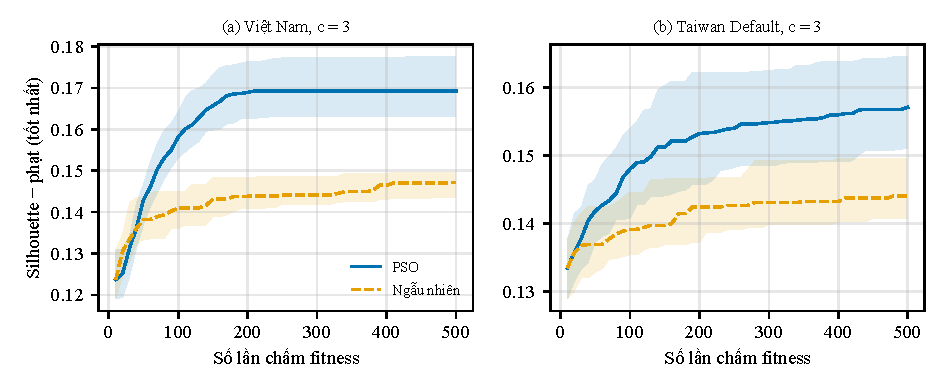
\includegraphics[width=\linewidth]{e8-hoi-tu}
\caption{TN3: fitness tốt nhất (Silhouette trừ phạt cụm nhỏ) theo số lần tính fitness của PSO và tìm ngẫu nhiên; đường là
trung vị, dải là khoảng tứ phân vị của 30 seed}
\label{fig:e8-hoi-tu}
\end{figure}

WFCM giải tích rẻ hơn khoảng hai bậc độ lớn và trên Việt Nam với $c = 3$,
$c = 4$ cho AUC và $\Delta r$ ngang hoặc hơn PSO. Nhưng trên Taiwan Default với $c = 3$, công thức gần như làm mất khả năng
tách rủi ro (AUC \soLieuETamTaiwanKiemChungCBaWfcmGiaiTichAucCung, $\Delta r$
\soLieuETamTaiwanKiemChungCBaWfcmGiaiTichChenhTiLe), trong khi PSO đạt \soLieuETamTaiwanKiemChungCBaPsoTrongSoAucCung{} và
\soLieuETamTaiwanKiemChungCBaPsoTrongSoChenhTiLe. Công thức dồn trọng số vào thuộc tính làm các cụm chặt nhất; trên Taiwan
Default đó là dư nợ các tháng (BILL\_AMT2--6, seed 1000), đúng nhóm mà PSO giảm trọng số (Hình~\ref{fig:e8-trong-so}). Tính
trên cả 7 bộ, PSO tốt hơn WFCM giải tích ở \soLieuETamAucCungWfcmGiaiTichHon{} cấu hình và kém ở
\soLieuETamAucCungWfcmGiaiTichKem{} cấu hình theo AUC; không cách nào thắng ở mọi bộ.

Các đối chứng trên đều là FCM với $m = 2$, mà với $c \ge 3$ FCM này gần suy biến (mục~\ref{sec:vi-sao}). Vì vậy nhóm chạy
thêm K-means không trọng số, cùng seed và tiền xử lý, làm mốc tham chiếu (Bảng~\ref{tab:e8-kmeans}; Holm riêng trên
\soLieuETamKmSoPhep{} phép so để không đổi họ kiểm định của TN3). Với 2 cụm, PSO tốt hơn K-means trên cả 2 bộ chính. Với
3 và 4 cụm, K-means tách rủi ro tốt hơn: trên Việt Nam, $\Delta r$ với $c = 4$ là \soLieuETamKmVietNamCBonChenhTiLe{} so
với \soLieuETamVietNamCBonPsoTrongSoChenhTiLe{} của PSO; trên Taiwan Default, K-means hơn có ý nghĩa ở $\Delta r$ với $c = 4$,
còn với $c = 3$ không phát hiện khác biệt. Tính trên 7 bộ, PSO tốt hơn / không khác / kém K-means ở
\soLieuETamKmChenhTiLeHon{} / \soLieuETamKmChenhTiLeBang{} / \soLieuETamKmChenhTiLeKem{} cấu hình theo $\Delta r$. Như vậy lợi
ích của PSO tìm trọng số là lợi ích so với FCM $m = 2$, chưa phải so với mọi cách phân cụm; khi chỉ cần phân hoạch cứng,
K-means là mốc phải so trước. Lý do giữ FCM nằm ở độ thuộc (mục~\ref{sec:dien-giai}).

\begin{table}[htbp]
\centering
\caption{TN3 -- K-means không trọng số làm mốc tham chiếu trên 2 bộ chính}
\label{tab:e8-kmeans}
\footnotesize
\setlength{\tabcolsep}{3pt}
\begin{tabular}{@{}llrrrrrr@{}}
\toprule
& & \multicolumn{3}{c}{AUC phân hoạch} & \multicolumn{3}{c}{Chênh tỉ lệ vỡ nợ} \\
\cmidrule(lr){3-5} \cmidrule(lr){6-8}
Bộ dữ liệu & c & FCM & K-means & PSO & FCM & K-means & PSO \\
\midrule
Việt Nam & 2 & 0,799 & 0,843 & 0,850\textsuperscript{+} & 0,284 & 0,373 & 0,438\textsuperscript{+} \\
 & 3 & 0,834 & 0,879 & 0,844\textsuperscript{--} & 0,341 & 0,563 & 0,465\textsuperscript{--} \\
 & 4 & 0,863 & 0,882 & 0,876\textsuperscript{--} & 0,420 & 0,842 & 0,557\textsuperscript{--} \\
\midrule
Taiwan Default & 2 & 0,523 & 0,504 & 0,517\textsuperscript{+} & 0,036 & 0,007 & 0,033\textsuperscript{+} \\
 & 3 & 0,601 & 0,699 & 0,664 & 0,155 & 0,385 & 0,261 \\
 & 4 & 0,526 & 0,684 & 0,645 & 0,168 & 0,446 & 0,315\textsuperscript{--} \\
\bottomrule
\end{tabular}
\par\smallskip\parbox{\linewidth}{\scriptsize Ghi chú: Trung vị 30 seed, cùng seed và tiền xử lý với Bảng~\ref{tab:e8-ket-qua}. FCM: FCM k-means++, m = 2; PSO: FCM với trọng số do PSO tìm. Dấu \textsuperscript{+} / \textsuperscript{--}: PSO tốt hơn / kém hơn K-means có ý nghĩa (Wilcoxon theo cặp seed, Holm trên 42 phép so với K-means ở 7 bộ, $\alpha = 0{,}05$).}
\end{table}


\subsection{Trọng số tìm được và chi phí}

Hình~\ref{fig:e8-trong-so} cho thấy PSO chọn các thuộc tính có nghĩa kinh tế rõ. Trên Taiwan
Default, 3 thuộc tính nặng nhất là \soLieuETamTaiwanKiemChungTrongSoCaoMotTen, \soLieuETamTaiwanKiemChungTrongSoCaoHaiTen{} và
\soLieuETamTaiwanKiemChungTrongSoCaoBaTen{} (tình trạng trả nợ các tháng), trùng với trục phân cụm đọc được ở
mục~\ref{sec:dien-giai}, còn hạn mức và dư nợ các tháng bị giảm trọng số. Trên Việt Nam, trọng số dồn vào các tỉ số định giá
(\soLieuETamVietNamTrongSoCaoMotTen: EV/doanh thu; \soLieuETamVietNamTrongSoCaoBaTen: P/S) và đòn bẩy
(\soLieuETamVietNamTrongSoCaoHaiTen: tổng nợ/vốn chủ sở hữu), mỗi thuộc tính nặng gấp khoảng
\soLieuETamVietNamTrongSoCaoMotGiaTri{} lần trung bình, còn các tỉ số thanh khoản (X1, X2) và phần lớn tỉ số thị trường khác
bị đẩy về gần cận dưới. Vector trọng số vì vậy còn cho biết nhóm chỉ tiêu nào quyết định phân khúc.

\begin{figure}[htbp]
\centering
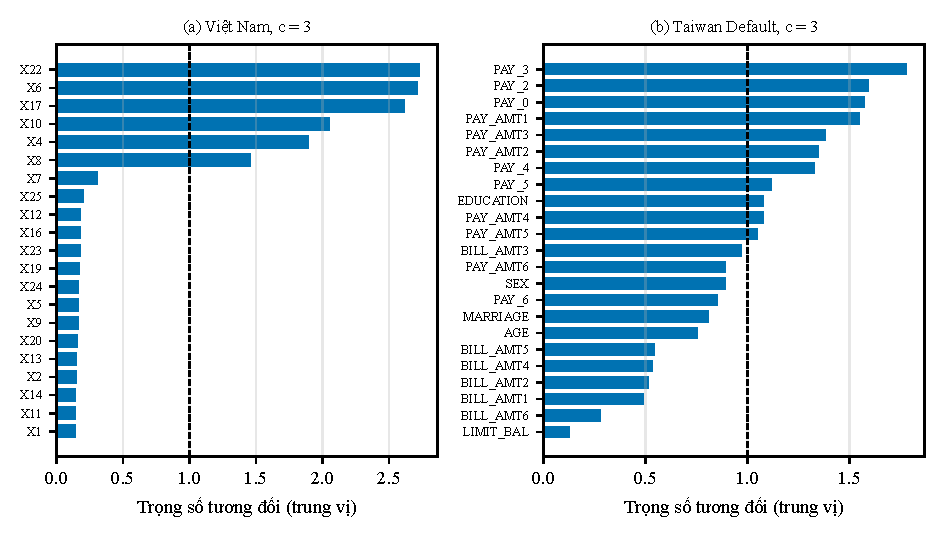
\includegraphics[width=\linewidth]{e8-trong-so}
\caption{TN3: trọng số tương đối (chia cho trung bình, trung vị của 30 seed) do PSO tìm với $c = 3$; đường đứt là trọng số
bằng nhau của FCM thường}
\label{fig:e8-trong-so}
\end{figure}

Một lượt PSO tìm trọng số mất khoảng \soLieuETamThoiGianPso{} giây (trung vị trên mọi cấu hình), so với
\soLieuETamThoiGianFcm{} giây của FCM thường, vì mỗi lần tính fitness là một lần chạy FCM và một lần tính Silhouette. Chi phí
này chỉ trả một lần khi dựng phân khúc, nên chấp nhận được với dữ liệu cỡ vài nghìn khách hàng; với dữ liệu lớn hơn cần giảm
mẫu Silhouette hoặc trần vòng FCM bên trong.


% Hà; Hải — QPSO và chi phí
\section{Năm phiên bản PSO khi tìm trọng số}
\label{sec:phien-ban-trong-so}

Mục này trả lời CH3 bằng TN4: 5 phiên bản PSO (Bảng~\ref{tab:ch2-phien-ban}) lắp vào cùng khung tìm trọng số
(Thuật toán~\ref{alg:pso-trong-so}), chạy trên 2 bộ chính với $c = 2, 3, 4$ ở 2 ngân sách, 500 lần tính fitness (10 hạt) và
1.000 lần (20 hạt), cùng 49 vòng (\soLieuEChinSoLuot{} lượt). Mỗi phiên bản được so với tìm ngẫu nhiên cùng ngân sách và mỗi
bản cải tiến được so với PSO gốc, trên điểm fitness (Silhouette trừ phạt), AUC phân hoạch và chênh tỉ lệ vỡ nợ, ở
\soLieuEChinSoO{} ô (2 bộ, 3 số cụm, 2 ngân sách); Holm hiệu chỉnh trên cả \soLieuEChinSoPhep{} phép so
(Bảng~\ref{tab:e9-tong-hop}--\ref{tab:e9-chenh}, Hình~\ref{fig:e9-quy-dao}).

\begin{table}[htbp]
\centering
\caption{TN4 -- số ô mỗi phiên bản tốt hơn / không khác / kém hơn tìm ngẫu nhiên và PSO gốc}
\label{tab:e9-tong-hop}
\footnotesize
\setlength{\tabcolsep}{3pt}
\begin{tabular}{@{}lcccccc@{}}
\toprule
& \multicolumn{3}{c}{So với tìm ngẫu nhiên} & \multicolumn{3}{c}{So với PSO gốc} \\
\cmidrule(lr){2-4} \cmidrule(lr){5-7}
Phiên bản & Điểm & AUC & $\Delta r$ & Điểm & AUC & $\Delta r$ \\
\midrule
Gốc & 11/1/0 & 2/10/0 & 9/3/0 & -- & -- & -- \\
W & 11/1/0 & 3/9/0 & 8/4/0 & 0/12/0 & 0/12/0 & 0/12/0 \\
S & 12/0/0 & 1/11/0 & 8/4/0 & 0/12/0 & 0/12/0 & 0/12/0 \\
LOG & 11/1/0 & 3/9/0 & 8/4/0 & 0/12/0 & 0/12/0 & 0/12/0 \\
QPSO & 12/0/0 & 4/8/0 & 9/3/0 & 0/12/0 & 0/12/0 & 0/12/0 \\
\bottomrule
\end{tabular}
\par\smallskip\parbox{\linewidth}{\scriptsize Ghi chú: 12 ô (2 bộ × 3 số cụm × 2 ngân sách). Điểm: Silhouette − phạt (chính là fitness); Wilcoxon theo cặp seed, Holm toàn họ, $\alpha = 0{,}05$.}
\end{table}


\subsection{Mọi phiên bản đều hơn tìm ngẫu nhiên}

Cả 5 phiên bản cho điểm fitness tốt hơn tìm ngẫu nhiên cùng ngân sách có ý nghĩa ở \soLieuEChinGocNgauNhienDiemHon{} đến
12 trên \soLieuEChinSoO{} ô, và chênh tỉ lệ vỡ nợ tốt hơn ở 8 đến 9 ô; không phiên bản nào kém tìm ngẫu nhiên ở ô nào, trên
chỉ số nào. Với AUC phân hoạch, phần lớn ô không khác (Bảng~\ref{tab:e9-tong-hop}): trên Việt Nam, mọi cách đánh trọng số đều
đã nâng AUC so với FCM thường, và khác biệt giữa PSO và tìm ngẫu nhiên nằm ở mức tách của cụm rủi ro cao, tức $\Delta r$. Hình~\ref{fig:e9-quy-dao}
cho thấy cách khoảng cách hình thành: mọi phiên bản tăng nhanh trong 200--400 lần tính fitness đầu rồi chững lại, còn tìm ngẫu
nhiên chỉ tăng chậm sau khoảng 200 lần. Theo trung vị, PSO với 500 lần đã có điểm cao hơn tìm ngẫu nhiên với 1.000 lần ở mọi ô;
chẳng hạn trên Việt
Nam với $c = 3$, điểm của PSO-W với 500 lần là \soLieuEChinVietNamCBaPsoWNamKhongKhongDiem{} so với
\soLieuEChinVietNamCBaNgauNhienMotKhongKhongKhongDiem{} của tìm ngẫu nhiên với 1.000 lần. Kết quả này củng cố TN3: phần lợi ích
do cơ chế bầy đàn không phụ thuộc phiên bản PSO nào được chọn.

\begin{table}[htbp]
\centering
\caption{TN4 -- Silhouette − phạt của 5 phiên bản PSO khi tìm trọng số thuộc tính}
\label{tab:e9-diem}
\footnotesize
\setlength{\tabcolsep}{3pt}
\begin{tabular}{@{}lllrrrrrrr@{}}
\toprule
Bộ dữ liệu & c & Ngân sách & FCM & NN & Gốc & W & S & LOG & QPSO \\
\midrule
Việt Nam & 2 & 500 & -- & 0,260 & 0,293\textsuperscript{+} & \textbf{0,296\textsuperscript{+}} & 0,292\textsuperscript{+} & \textbf{0,296\textsuperscript{+}} & 0,295\textsuperscript{+} \\
 &  & 1.000 &  & 0,263 & 0,296\textsuperscript{+} & 0,298\textsuperscript{+} & 0,295\textsuperscript{+} & 0,294\textsuperscript{+} & \textbf{0,303\textsuperscript{+}} \\
 & 3 & 500 & -- & 0,147 & 0,167\textsuperscript{+} & 0,169\textsuperscript{+} & 0,169\textsuperscript{+} & 0,170\textsuperscript{+} & \textbf{0,172\textsuperscript{+}} \\
 &  & 1.000 &  & 0,148 & 0,177\textsuperscript{+} & 0,175\textsuperscript{+} & 0,176\textsuperscript{+} & \textbf{0,180\textsuperscript{+}} & \textbf{0,180\textsuperscript{+}} \\
 & 4 & 500 & -- & 0,104 & 0,132\textsuperscript{+} & 0,133\textsuperscript{+} & 0,130\textsuperscript{+} & \textbf{0,135\textsuperscript{+}} & 0,130\textsuperscript{+} \\
 &  & 1.000 &  & 0,106 & 0,131\textsuperscript{+} & 0,134\textsuperscript{+} & 0,131\textsuperscript{+} & 0,132\textsuperscript{+} & \textbf{0,136\textsuperscript{+}} \\
\midrule
Taiwan Default & 2 & 500 & -- & 0,310 & 0,328\textsuperscript{+} & 0,329\textsuperscript{+} & 0,329\textsuperscript{+} & 0,331\textsuperscript{+} & \textbf{0,331\textsuperscript{+}} \\
 &  & 1.000 &  & 0,310 & 0,332\textsuperscript{+} & 0,331\textsuperscript{+} & 0,330\textsuperscript{+} & 0,332\textsuperscript{+} & \textbf{0,333\textsuperscript{+}} \\
 & 3 & 500 & -- & 0,144 & \textbf{0,160\textsuperscript{+}} & 0,157\textsuperscript{+} & 0,158\textsuperscript{+} & 0,159\textsuperscript{+} & 0,154\textsuperscript{+} \\
 &  & 1.000 &  & 0,144 & 0,163\textsuperscript{+} & 0,163\textsuperscript{+} & \textbf{0,165\textsuperscript{+}} & 0,164\textsuperscript{+} & 0,161\textsuperscript{+} \\
 & 4 & 500 & -- & 0,126 & 0,133 & 0,135 & \textbf{0,138\textsuperscript{+}} & 0,135 & 0,137\textsuperscript{+} \\
 &  & 1.000 &  & 0,129 & 0,145\textsuperscript{+} & 0,143\textsuperscript{+} & 0,148\textsuperscript{+} & 0,144\textsuperscript{+} & \textbf{0,150\textsuperscript{+}} \\
\bottomrule
\end{tabular}
\par\smallskip\parbox{\linewidth}{\scriptsize Ghi chú: Trung vị 30 seed, m = 2; ngân sách là số lần tính fitness (10 hạt với 500, 20 hạt với 1.000). NN: tìm ngẫu nhiên cùng ngân sách. Đậm: cao nhất trong các phương pháp tìm kiếm cùng ngân sách. \textsuperscript{+} / \textsuperscript{--}: tốt hơn / kém hơn NN có ý nghĩa; \textsuperscript{*} / \textsuperscript{\dag}: tốt hơn / kém hơn PSO gốc có ý nghĩa (Wilcoxon theo cặp seed, Holm toàn họ, $\alpha = 0{,}05$).}
\end{table}


\begin{figure}[htbp]
\centering
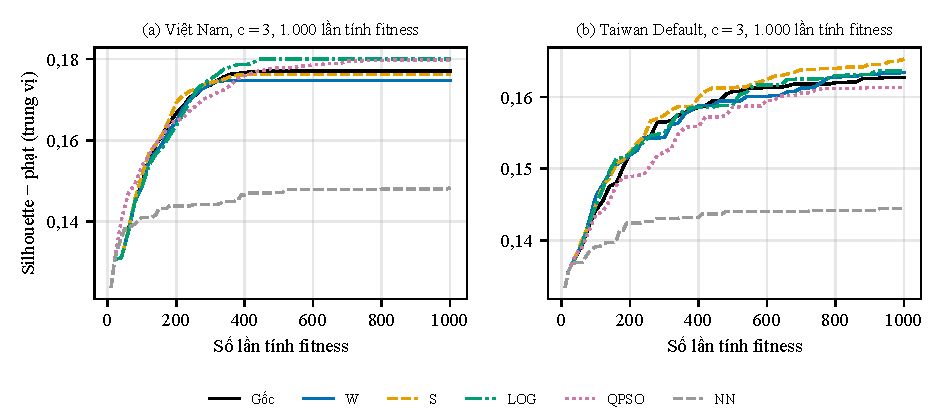
\includegraphics[width=\linewidth]{e9-quy-dao}
\caption{TN4: điểm fitness tốt nhất (Silhouette trừ phạt, trung vị 30 seed) theo số lần tính fitness của 5 phiên bản PSO
và tìm ngẫu nhiên (NN), ngân sách 1.000 lần, $c = 3$}
\label{fig:e9-quy-dao}
\end{figure}

\subsection{Các bản cải tiến không hơn PSO gốc}

Không bản cải tiến nào khác PSO gốc có ý nghĩa ở bất kỳ ô nào, trên cả 3 chỉ số (Bảng~\ref{tab:e9-tong-hop}); trên hình,
quỹ đạo của 5 phiên bản gần như chồng lên nhau. QPSO là bản gần ngưỡng nhất, với trung vị $\Delta r$ cao hơn trên Taiwan Default
$c = 4$ (Bảng~\ref{tab:e9-chenh}) nhưng không còn ý nghĩa sau hiệu chỉnh. Kết quả này ngược với phần tìm tâm, nơi cả 4 bản cải
tiến đều đưa gbest gần cực tiểu hơn PSO gốc (mục~\ref{sec:e5-dat-j}). Một cách giải thích là khác biệt về không gian tìm kiếm:
khi tìm tâm, hộp tìm kiếm rộng bằng miền dữ liệu và PSO gốc ($\omega = 1$) không thu hẹp được quanh gbest; khi tìm trọng số,
hộp chỉ là $[0{,}05;\ 1]^D$ và fitness thay đổi theo bậc, vì nhiều vector trọng số gần nhau cho cùng một phân hoạch cứng, nên
việc thu hẹp bước đi không đem lại thêm bao nhiêu. Nhóm không có phép thử tách riêng nguyên nhân này.

\begin{table}[htbp]
\centering
\caption{TN4 -- Chênh tỉ lệ vỡ nợ của 5 phiên bản PSO khi tìm trọng số thuộc tính}
\label{tab:e9-chenh}
\footnotesize
\setlength{\tabcolsep}{3pt}
\begin{tabular}{@{}lllrrrrrrr@{}}
\toprule
Bộ dữ liệu & c & Ngân sách & FCM & NN & Gốc & W & S & LOG & QPSO \\
\midrule
Việt Nam & 2 & 500 & 0,284 & 0,356 & 0,436\textsuperscript{+} & 0,438\textsuperscript{+} & 0,425\textsuperscript{+} & \textbf{0,447\textsuperscript{+}} & 0,442\textsuperscript{+} \\
 &  & 1.000 &  & 0,363 & 0,447\textsuperscript{+} & 0,438\textsuperscript{+} & 0,446\textsuperscript{+} & 0,441\textsuperscript{+} & \textbf{0,456\textsuperscript{+}} \\
 & 3 & 500 & 0,341 & 0,415 & 0,460\textsuperscript{+} & 0,465\textsuperscript{+} & 0,467\textsuperscript{+} & \textbf{0,468\textsuperscript{+}} & 0,462\textsuperscript{+} \\
 &  & 1.000 &  & 0,415 & 0,473\textsuperscript{+} & 0,471\textsuperscript{+} & \textbf{0,475\textsuperscript{+}} & 0,470\textsuperscript{+} & 0,474\textsuperscript{+} \\
 & 4 & 500 & 0,420 & 0,498 & 0,541\textsuperscript{+} & \textbf{0,557} & 0,544 & 0,536 & 0,552\textsuperscript{+} \\
 &  & 1.000 &  & 0,507 & 0,553\textsuperscript{+} & 0,549\textsuperscript{+} & 0,567\textsuperscript{+} & 0,559\textsuperscript{+} & \textbf{0,572\textsuperscript{+}} \\
\midrule
Taiwan Default & 2 & 500 & 0,036 & 0,009 & 0,031\textsuperscript{+} & \textbf{0,033\textsuperscript{+}} & 0,026\textsuperscript{+} & 0,030\textsuperscript{+} & 0,032\textsuperscript{+} \\
 &  & 1.000 &  & 0,010 & 0,031\textsuperscript{+} & \textbf{0,032\textsuperscript{+}} & 0,031\textsuperscript{+} & \textbf{0,032\textsuperscript{+}} & \textbf{0,032\textsuperscript{+}} \\
 & 3 & 500 & 0,155 & 0,238 & 0,261 & \textbf{0,261} & 0,258 & 0,257 & \textbf{0,261} \\
 &  & 1.000 &  & 0,241 & 0,270\textsuperscript{+} & 0,272\textsuperscript{+} & 0,271\textsuperscript{+} & \textbf{0,274\textsuperscript{+}} & 0,257 \\
 & 4 & 500 & 0,168 & 0,266 & 0,302 & 0,315 & 0,299 & 0,274 & \textbf{0,345\textsuperscript{+}} \\
 &  & 1.000 &  & 0,277 & 0,287 & 0,283 & 0,319 & 0,282 & \textbf{0,358} \\
\bottomrule
\end{tabular}
\par\smallskip\parbox{\linewidth}{\scriptsize Ghi chú: Trung vị 30 seed, m = 2; ngân sách là số lần tính fitness (10 hạt với 500, 20 hạt với 1.000). NN: tìm ngẫu nhiên cùng ngân sách. Đậm: cao nhất trong các phương pháp tìm kiếm cùng ngân sách. \textsuperscript{+} / \textsuperscript{--}: tốt hơn / kém hơn NN có ý nghĩa; \textsuperscript{*} / \textsuperscript{\dag}: tốt hơn / kém hơn PSO gốc có ý nghĩa (Wilcoxon theo cặp seed, Holm toàn họ, $\alpha = 0{,}05$).}
\end{table}


Tăng ngân sách từ 500 lên 1.000 lần tính fitness làm trung vị điểm fitness tốt lên ở 27 trên 30 trường hợp (5 phiên bản,
6 cấu hình), rõ nhất khi có nhiều cụm (trên Taiwan
Default với $c = 4$, PSO gốc từ \soLieuEChinTaiwanKiemChungCBonPsoGocNamKhongKhongDiem{} lên
\soLieuEChinTaiwanKiemChungCBonPsoGocMotKhongKhongKhongDiem), nhưng không đổi kết luận về $\Delta r$ và AUC, trong khi thời gian
gấp đôi (trung vị \soLieuEChinVietNamCBaPsoWNamKhongKhongTTong~s với PSO-W 500 lần trên Việt Nam $c = 3$). Không phát hiện khác
biệt giữa các phiên bản sau hiệu chỉnh Holm; vì họ hiệu chỉnh gộp nhiều phép so nên kiểm định kém nhạy, và kết quả âm này chỉ cho thấy
khác biệt (nếu có) là nhỏ. Về thực hành, PSO gốc hoặc PSO-W với khoảng 500 lần tính fitness là đủ.

% Bình
\section{Kiểm chứng trên mẫu độc lập và giới hạn}
\label{sec:kiem-chung}

Mục này trả lời CH4 và là bước 3 của quy trình đề xuất. Ở TN3, trọng số được tìm và đánh giá trên cùng một mẫu; nếu PSO chỉ
khớp với đặc điểm riêng của mẫu đó, lợi ích sẽ không giữ khi áp trọng số lên khách hàng mới. TN5 học trọng số trên một mẫu
nguồn, rồi trên một mẫu đích độc lập chạy FCM với trọng số đó từ cùng tâm khởi tạo k-means++ như FCM thường. Có 4 chiều
chuyển: 2 mẫu 5.000 khách hàng không giao nhau của Taiwan Default theo cả 2 chiều, và 2 nửa của bộ Việt Nam chia theo
doanh nghiệp theo cả 2 chiều. Mỗi chiều so 5 cách trên mẫu đích: FCM thường, trọng số chuyển từ WFCM giải tích, từ tìm
ngẫu nhiên, từ PSO-W, và PSO-W học ngay trên mẫu đích làm mốc ``tại chỗ'' (Bảng~\ref{tab:e10-ket-qua},
\ref{tab:e10-tong-hop}; \soLieuEMuoiSoLuot{} lượt).

\begin{table}[htbp]
\centering
\caption{TN5 -- trọng số học trên mẫu nguồn, áp lên mẫu đích độc lập}
\label{tab:e10-ket-qua}
\footnotesize
\setlength{\tabcolsep}{2pt}
\begin{tabular}{@{}llrrrrrrrrrr@{}}
\toprule
& & \multicolumn{5}{c}{AUC phân hoạch trên mẫu đích} & \multicolumn{5}{c}{Chênh tỉ lệ vỡ nợ trên mẫu đích} \\
\cmidrule(lr){3-7} \cmidrule(lr){8-12}
Chiều chuyển & c & FCM & WFCM & NN & PSO & Tại chỗ & FCM & WFCM & NN & PSO & Tại chỗ \\
\midrule
Taiwan: thiết kế → kiểm chứng & 2 & \textbf{0,523\textsuperscript{--}} & 0,515 & 0,505\textsuperscript{+} & 0,516 & 0,517 & \textbf{0,036} & 0,024 & 0,008\textsuperscript{+} & 0,030 & 0,033 \\
 & 3 & 0,601\textsuperscript{+} & 0,510\textsuperscript{+} & 0,634 & 0,646 & \textbf{0,664\textsuperscript{--}} & 0,155\textsuperscript{+} & 0,015\textsuperscript{+} & 0,212 & 0,232 & \textbf{0,261\textsuperscript{--}} \\
 & 4 & 0,526\textsuperscript{+} & 0,583 & 0,639 & 0,572 & \textbf{0,645\textsuperscript{--}} & 0,168 & 0,154\textsuperscript{+} & 0,268 & 0,292 & \textbf{0,315} \\
\midrule
Taiwan: kiểm chứng → thiết kế & 2 & 0,509\textsuperscript{+} & 0,500\textsuperscript{+} & 0,521\textsuperscript{+} & \textbf{0,530} & \textbf{0,531} & 0,014\textsuperscript{+} & 0,000\textsuperscript{+} & 0,034\textsuperscript{+} & 0,057 & \textbf{0,059} \\
 & 3 & 0,604\textsuperscript{+} & 0,532\textsuperscript{+} & 0,648 & \textbf{0,653} & 0,650 & 0,160\textsuperscript{+} & 0,048\textsuperscript{+} & 0,226 & \textbf{0,244} & 0,240 \\
 & 4 & 0,525\textsuperscript{+} & 0,617\textsuperscript{+} & 0,644 & \textbf{0,647} & 0,585 & 0,080\textsuperscript{+} & 0,193 & 0,234 & \textbf{0,252} & 0,243 \\
\midrule
Việt Nam: nửa 0 → nửa 1 & 2 & 0,793\textsuperscript{+} & 0,802\textsuperscript{+} & 0,832 & 0,827 & \textbf{0,840} & 0,282\textsuperscript{+} & 0,313\textsuperscript{+} & 0,356\textsuperscript{+} & 0,437 & \textbf{0,442} \\
 & 3 & 0,823 & \textbf{0,835\textsuperscript{--}} & 0,830 & 0,820 & 0,828 & 0,345\textsuperscript{+} & \textbf{0,482} & 0,408\textsuperscript{+} & 0,456 & 0,468 \\
 & 4 & 0,840 & 0,850 & \textbf{0,856} & 0,851 & 0,851 & 0,393\textsuperscript{+} & \textbf{0,613} & 0,489\textsuperscript{+} & 0,517 & 0,588 \\
\midrule
Việt Nam: nửa 1 → nửa 0 & 2 & 0,817\textsuperscript{+} & 0,829\textsuperscript{+} & 0,854\textsuperscript{+} & 0,865 & \textbf{0,870} & 0,295\textsuperscript{+} & 0,311\textsuperscript{+} & 0,362\textsuperscript{+} & 0,417 & \textbf{0,437} \\
 & 3 & 0,855\textsuperscript{+} & \textbf{0,884} & 0,877 & 0,877 & 0,876 & 0,354\textsuperscript{+} & 0,475 & 0,427\textsuperscript{+} & 0,482 & \textbf{0,486} \\
 & 4 & 0,884\textsuperscript{+} & 0,894\textsuperscript{+} & 0,901 & \textbf{0,901} & 0,900 & 0,432\textsuperscript{+} & \textbf{0,622} & 0,518\textsuperscript{+} & 0,584 & 0,548 \\
\bottomrule
\end{tabular}
\par\smallskip\parbox{\linewidth}{\scriptsize Ghi chú: Trung vị 30 seed, m = 2. FCM: trọng số bằng nhau; WFCM, NN, PSO: trọng số học trên mẫu nguồn bằng WFCM giải tích, tìm ngẫu nhiên và PSO-W; Tại chỗ: PSO-W học ngay trên mẫu đích. Mọi cột dùng cùng tâm khởi tạo k-means++ trên mẫu đích. Đậm: cao nhất hàng. Dấu \textsuperscript{+} / \textsuperscript{--} sau một cột: PSO chuyển tốt hơn / kém hơn cột đó có ý nghĩa (Wilcoxon theo cặp seed, Holm toàn họ, $\alpha = 0{,}05$).}
\end{table}


\begin{table}[htbp]
\centering
\caption{TN5 -- số cấu hình trọng số PSO chuyển sang mẫu đích tốt hơn / không khác / kém hơn từng cách khác}
\label{tab:e10-tong-hop}
\footnotesize
\setlength{\tabcolsep}{3pt}
\begin{tabular}{@{}lcccc@{}}
\toprule
PSO chuyển so với & FCM & WFCM chuyển & NN chuyển & PSO tại chỗ \\
\midrule
AUC phân hoạch & 9 / 2 / 1 & 7 / 4 / 1 & 3 / 9 / 0 & 0 / 10 / 2 \\
Chênh tỉ lệ vỡ nợ & 10 / 2 / 0 & 6 / 6 / 0 & 8 / 4 / 0 & 0 / 11 / 1 \\
Silhouette − phạt & 12 / 0 / 0 & 10 / 2 / 0 & 9 / 3 / 0 & 0 / 7 / 5 \\
\bottomrule
\end{tabular}
\par\smallskip\parbox{\linewidth}{\scriptsize Ghi chú: 12 cấu hình (4 chiều chuyển × 3 số cụm), Wilcoxon theo cặp seed, Holm toàn họ, $\alpha = 0{,}05$.}
\end{table}


\subsection{Lợi ích giữ trên mẫu độc lập}

Trọng số PSO học trên mẫu nguồn vẫn làm FCM tách rủi ro tốt hơn FCM thường trên mẫu đích: tốt hơn có ý nghĩa ở
\soLieuEMuoiChenhTiLeFcmKppHon{} trên \soLieuEMuoiSoCauHinh{} cấu hình theo chênh tỉ lệ vỡ nợ (không cấu hình nào kém hơn) và
\soLieuEMuoiAucCungFcmKppHon{} cấu hình theo AUC phân hoạch. Trên Việt Nam (nửa 0 sang nửa 1, $c = 2$), $\Delta r$ tăng từ
\soLieuEMuoiVnKhongMotCHaiFcmKppChenhTiLe{} lên \soLieuEMuoiVnKhongMotCHaiPsoChuyenChenhTiLe; trên Taiwan Default (mẫu kiểm
chứng sang mẫu thiết kế, $c = 4$), AUC tăng từ \soLieuEMuoiTaiwanKcTkCBonFcmKppAucCung{} lên
\soLieuEMuoiTaiwanKcTkCBonPsoChuyenAucCung. Cấu hình duy nhất kém hơn FCM thường (theo AUC, không theo $\Delta r$) là Taiwan
Default với $c = 2$ (mẫu thiết kế sang mẫu kiểm chứng), đúng chỗ PSO đã yếu ở TN3.

So với PSO học ngay trên mẫu đích, trọng số chuyển sang không khác có ý nghĩa ở \soLieuEMuoiChenhTiLePsoTaiChoBang{} cấu hình
theo $\Delta r$ và \soLieuEMuoiAucCungPsoTaiChoBang{} cấu hình theo AUC. Phần mất đi tập trung ở một chiều chuyển của Taiwan
Default (mẫu thiết kế sang mẫu kiểm chứng) với $c = 3, 4$; chẳng hạn với $c = 4$, AUC là
\soLieuEMuoiTaiwanTkKcCBonPsoChuyenAucCung{} so với \soLieuEMuoiTaiwanTkKcCBonPsoTaiChoAucCung{} khi học tại chỗ, vẫn cao hơn FCM
thường. Trọng số học ở 2 mẫu cũng giống nhau: cosine trung vị giữa trọng số học trên mẫu nguồn và trên mẫu đích là
\soLieuEMuoiTaiwanTkKcCosTrongSo{} ở Taiwan Default và \soLieuEMuoiVnKhongMotCosTrongSo{} ở Việt Nam. Tuy vậy, do mọi trọng số đều dương,
hai vector ngẫu nhiên trong miền tìm kiếm cũng có cosine khoảng 0,8, nên con số này chưa cho thấy từng giá trị trọng số ổn
định giữa 2 mẫu; thứ giữ được là lợi ích của phân hoạch.

Phần lợi ích do cơ chế bầy đàn cũng giữ: trọng số PSO chuyển sang tốt hơn trọng số tìm ngẫu nhiên chuyển sang ở
\soLieuEMuoiChenhTiLeNgauNhienChuyenHon{} cấu hình theo $\Delta r$ (không cấu hình nào kém hơn), rõ nhất trên Việt Nam ở mọi
chiều và mọi $c$. So với WFCM giải tích chuyển sang, PSO tốt hơn ở \soLieuEMuoiChenhTiLeWfcmChuyenHon{} cấu hình theo $\Delta r$
và \soLieuEMuoiAucCungWfcmChuyenHon{} cấu hình theo AUC; trên Taiwan Default công thức lại gần như xoá khả năng tách rủi ro
($\Delta r$ \soLieuEMuoiTaiwanTkKcCBaWfcmChuyenChenhTiLe{} với $c = 3$), giống TN3.

\subsection{Khi nào PSO tìm trọng số không có ích}
\label{sec:khong-co-ich}

Trên 7 bộ của TN3, PSO kém FCM thường có ý nghĩa ở \soLieuETamAucCungFcmKppKem{} cấu hình theo AUC, đều với
$c = 2$ (Australian, Polish, South German, Taiwan Bankruptcy, Taiwan Default). Với 2 cụm, FCM thường đã tách theo trục có
liên quan tới vỡ nợ, còn PSO tìm một cách tách đẹp hơn về hình học (Silhouette cao hơn) nhưng ít liên quan tới rủi ro hơn:
fitness không nhìn nhãn nên không có gì bảo đảm 2 mục tiêu trùng nhau. Ở Australian, South German và Taiwan Bankruptcy với
$c \ge 3$ (và Polish với $c = 4$), FCM thường cho nghiệm gần sụp, cụm nhỏ nhất chỉ chiếm \soLieuETamSouthGermanCBaFcmKppCumNhoNhat{} dữ liệu (South
German, $c = 3$) hoặc \soLieuETamAustralianCBonFcmKppCumNhoNhat{} (Australian, $c = 4$). Phạt cụm nhỏ buộc PSO tìm phân hoạch
cân hơn; trên South German điều này làm AUC tăng (\soLieuETamSouthGermanCBonFcmKppAucCung{} lên
\soLieuETamSouthGermanCBonPsoTrongSoAucCung{} với $c = 4$), nhưng trên Australian và Polish thì không tăng có ý nghĩa. Trên
Taiwan Bankruptcy với $c = 4$, PSO giảm số cụm rỗng nhưng cụm nhỏ nhất vẫn dưới 0,1\% dữ liệu ở trung vị, tức phạt cụm nhỏ
không đạt được.

Tổng hợp TN3 và TN5, PSO tìm trọng số có ích khi dữ liệu có nhiều thuộc tính số liên tục đo các khía cạnh khác nhau của
rủi ro, như các tỉ số tài chính của bộ Việt Nam hay lịch sử trả nợ và dư nợ của bộ Taiwan Default: ở đó PSO có ích với mọi
$c$ đã thử trên Việt Nam và với $c = 3, 4$ trên Taiwan Default, còn $c = 2$ là chỗ yếu nhất. Trên các bộ mà đa số thuộc tính là mã thứ bậc hoặc định danh (South German,
German, Australian) hoặc có đuôi cực dài (2 bộ phá sản), FCM thường đã gần sụp và trọng số không cứu được. Vì fitness không
nhìn nhãn, bước 3 của quy trình đề xuất (mục~\ref{sec:de-xuat}) là cần thiết: dùng nhãn lịch sử trên một mẫu độc lập để quyết
định có áp trọng số hay không, đúng như TN5 làm.


\section{Diễn giải các phân khúc rủi ro}
\label{sec:dien-giai}

Mục này đọc các phân khúc với $c = 3$, $m = 2$, seed 1000, đặt phân hoạch FCM thường cạnh phân hoạch FCM có trọng số do
PSO-W tìm (TN3) trên cùng tâm khởi tạo (Bảng~\ref{tab:e4-profile-viet_nam}, \ref{tab:e4-profile-taiwan_kiem_chung}). Cụm được
đánh số theo tỉ lệ vỡ nợ tăng dần; cột ``mơ hồ'' là tỉ lệ khách hàng có độ thuộc lớn nhất dưới 0,6; 5 thuộc tính in ra (thang
gốc) là 5 thuộc tính có khoảng trung bình giữa các cụm của phân hoạch có trọng số rộng nhất, tính theo độ lệch chuẩn.

\begin{table}[htbp]
\centering
\caption{Profile cụm FCM thường và FCM có trọng số do PSO tìm trên Việt Nam (c = 3, seed 1000): trung bình giá trị gốc}
\label{tab:e4-profile-viet_nam}
\footnotesize
\setlength{\tabcolsep}{3pt}
\begin{tabular}{@{}lrrrrrrrrr@{}}
\toprule
Phương pháp & Cụm & Cỡ (\%) & Vỡ nợ (\%) & Mơ hồ (\%) & \rotatebox{60}{X17} & \rotatebox{60}{X11} & \rotatebox{60}{X6} & \rotatebox{60}{X10} & \rotatebox{60}{X8} \\
\midrule
FCM (k-means++) &1 & 40,9 & 1,3 & 100,0 & 2,09 & 0,19 & 0,24 & 0,26 & 0,22 \\
 &2 & 24,8 & 2,5 & 100,0 & 0,47 & 0,36 & 0,24 & 0,58 & 0,54 \\
 &3 & 34,3 & 35,4 & 90,7 & 0,39 & 0,67 & 1,28 & 2,54 & 2,13 \\
\midrule
PSO trọng số &1 & 56,6 & 3,1 & 17,6 & 0,51 & 0,34 & 0,29 & 0,65 & 0,60 \\
 &2 & 23,7 & 7,6 & 20,4 & 3,26 & 0,23 & 0,29 & 0,42 & 0,32 \\
 &3 & 19,6 & 49,8 & 26,7 & 0,24 & 0,73 & 1,86 & 3,34 & 2,74 \\
\bottomrule
\end{tabular}
\par\smallskip\parbox{\linewidth}{\scriptsize Ghi chú: cụm đánh số theo tỉ lệ vỡ nợ tăng dần; mơ hồ: tỉ lệ điểm trong cụm có độ thuộc lớn nhất $<$ 0,6; thuộc tính chọn là 5 thuộc tính có khoảng trung bình giữa các cụm (PSO trọng số) rộng nhất tính theo độ lệch chuẩn. X17: P/S; X11: phải trả người bán/tổng tài sản; X6: tổng nợ/VCSH; X10: phải trả người bán/VCSH; X8: nợ ngắn hạn/VCSH.}
\end{table}


Trên Việt Nam, trọng số làm phân khúc rủi ro cao gọn và rõ hơn. Với FCM thường, cụm rủi ro cao chiếm
\soLieuEBonVietNamFcmKppCumBaCo\% doanh nghiệp với tỉ lệ khó khăn tài chính \soLieuEBonVietNamFcmKppCumBaVoNo\%; với trọng số do PSO tìm,
cụm này chỉ còn \soLieuEBonVietNamPsoTrongSoCumBaCo\% doanh nghiệp nhưng tỉ lệ khó khăn tài chính lên \soLieuEBonVietNamPsoTrongSoCumBaVoNo\%,
còn cụm rủi ro thấp chiếm \soLieuEBonVietNamPsoTrongSoCumMotCo\% với tỉ lệ \soLieuEBonVietNamPsoTrongSoCumMotVoNo\%. Cụm rủi ro
cao có các tỉ số nợ trên vốn chủ sở hữu (X6, X8, X10) cao nhất, đúng các thuộc tính PSO đánh trọng số cao ở
Hình~\ref{fig:e8-trong-so}; tỉ số phải trả người bán trên tổng tài sản (X11) cũng cao dù trọng số của nó thấp. Cụm giữa được tách theo định giá: P/S (X17) cao gấp nhiều lần 2 cụm
còn lại, tức nhóm doanh nghiệp được thị trường định giá cao so với doanh thu, có tỉ lệ khó khăn tài chính \soLieuEBonVietNamPsoTrongSoCumHaiVoNo\%,
dưới mức chung của bộ dữ liệu. Độ thuộc cũng có ý nghĩa trở lại: tỉ lệ khách hàng mơ hồ giảm từ \soLieuEBonVietNamFcmKppCumBaMoHo--\soLieuEBonVietNamFcmKppCumMotMoHo\% ở FCM thường
xuống \soLieuEBonVietNamPsoTrongSoCumMotMoHo--\soLieuEBonVietNamPsoTrongSoCumBaMoHo\%, nên độ thuộc phân biệt được doanh nghiệp
điển hình với doanh nghiệp ``biên'', đúng lý do chọn phân cụm mờ ở Chương~\ref{chap:tong-quan}.

\begin{table}[htbp]
\centering
\caption{Profile cụm FCM thường và FCM có trọng số do PSO tìm trên Taiwan Default (c = 3, seed 1000): trung bình giá trị gốc}
\label{tab:e4-profile-taiwan_kiem_chung}
\footnotesize
\setlength{\tabcolsep}{3pt}
\begin{tabular}{@{}lrrrrrrrrr@{}}
\toprule
Phương pháp & Cụm & Cỡ (\%) & Vỡ nợ (\%) & Mơ hồ (\%) & \rotatebox{60}{PAY\_3} & \rotatebox{60}{PAY\_5} & \rotatebox{60}{PAY\_2} & \rotatebox{60}{PAY\_4} & \rotatebox{60}{PAY\_6} \\
\midrule
FCM (k-means++) &1 & 44,3 & 15,9 & 100,0 & −0,01 & −0,04 & −0,02 & −0,03 & −0,03 \\
 &2 & 25,1 & 21,7 & 75,1 & −1,16 & −1,36 & −1,06 & −1,30 & −1,44 \\
 &3 & 30,6 & 31,4 & 100,0 & 0,42 & 0,33 & 0,44 & 0,37 & 0,29 \\
\midrule
PSO trọng số &1 & 46,8 & 13,2 & 100,0 & −0,10 & −0,11 & −0,16 & −0,09 & −0,07 \\
 &2 & 27,0 & 20,4 & 86,2 & −1,25 & −1,36 & −1,13 & −1,32 & −1,40 \\
 &3 & 26,2 & 39,8 & 100,0 & 0,82 & 0,62 & 0,91 & 0,65 & 0,46 \\
\bottomrule
\end{tabular}
\par\smallskip\parbox{\linewidth}{\scriptsize Ghi chú: cụm đánh số theo tỉ lệ vỡ nợ tăng dần; mơ hồ: tỉ lệ điểm trong cụm có độ thuộc lớn nhất $<$ 0,6; thuộc tính chọn là 5 thuộc tính có khoảng trung bình giữa các cụm (PSO trọng số) rộng nhất tính theo độ lệch chuẩn. PAY\_k: tình trạng trả nợ ở tháng thứ k trước tháng quan sát (theo mô tả của UCI: $-1$ trả đúng hạn, $1$ đến $9$ trễ hạn 1 đến 9 tháng; dữ liệu còn các mã $-2$ và $0$ không được giải thích); giá trị dương là có trễ hạn.}
\end{table}


Trên Taiwan Default, trục phân khúc ở cả 2 phân hoạch là lịch sử trả nợ: 5 thuộc tính khác nhau nhiều nhất giữa các cụm đều
là tình trạng trả nợ các tháng (PAY\_2--PAY\_6), và cụm rủi ro cao gồm khách hàng có giá trị PAY dương, tức có trễ hạn. Trọng số
làm trục này rõ hơn: cụm rủi ro cao có PAY trung bình cao hơn và tỉ lệ vỡ nợ \soLieuEBonTaiwanKiemChungPsoTrongSoCumBaVoNo\%
(so với \soLieuEBonTaiwanKiemChungFcmKppCumBaVoNo\% ở FCM thường), còn cụm rủi ro thấp có tỉ lệ
\soLieuEBonTaiwanKiemChungPsoTrongSoCumMotVoNo\% (so với \soLieuEBonTaiwanKiemChungFcmKppCumMotVoNo\%). Khác với Việt Nam, độ
thuộc vẫn chia gần đều: tỉ lệ khách hàng mơ hồ ở 2 cụm vẫn là \soLieuEBonTaiwanKiemChungPsoTrongSoCumBaMoHo\%. Với $m = 2$, trọng
số làm phân hoạch cứng tách rủi ro tốt hơn nhưng chưa làm các tâm tách đủ xa để độ thuộc có ý nghĩa trên bộ này; chọn $m$ nhỏ
hơn (mục~\ref{sec:vi-sao}) là hướng bổ sung.

% Bình
\section{Đánh giá chung các thuật toán}
\label{sec:danh-gia-chung}

Các mục trên trả lời từng câu hỏi nghiên cứu. Mục này nhìn lại theo từng thuật toán: mỗi phiên bản PSO đã được dùng ở 2
vai trò, cùng với FCM, WFCM giải tích và tìm ngẫu nhiên làm đối chứng (Bảng~\ref{tab:ch3-danh-gia}).

\begin{table}[htbp]
\centering
\caption{Đánh giá các thuật toán trên dữ liệu tín dụng theo 2 vai trò}
\label{tab:ch3-danh-gia}
\footnotesize
\setlength{\tabcolsep}{3pt}
\renewcommand{\arraystretch}{1.15}
\begin{tabular}{@{}>{\raggedright\arraybackslash}p{2.3cm}>{\raggedright\arraybackslash}p{5.4cm}>{\raggedright\arraybackslash}p{5.0cm}>{\raggedright\arraybackslash}p{2.1cm}@{}}
\toprule
Thuật toán & Khi tìm tâm khởi tạo (TN1, TN2) & Khi tìm trọng số (TN3, TN4) & Thời gian \\
\midrule
FCM k-means++ & Đạt $J_m$ tốt nhất ở mọi lượt trên 2 bộ chính; chỉ kém PSO 2--3/30 seed ở một cấu hình nhiều cực tiểu & Mốc không trọng số; thua PSO
trên Việt Nam (mọi $c$) và Taiwan Default ($c = 3, 4$) & \soLieuETamThoiGianFcm~s \\
\addlinespace
WFCM giải tích & --- & Ngang hoặc hơn PSO trên Việt Nam $c = 3, 4$; gần như mất khả năng tách rủi ro trên Taiwan Default & cỡ một
lần FCM \\
\addlinespace
Tìm ngẫu nhiên & --- & Thua PSO về fitness ở \soLieuETamSilhouetteNgauNhienTrongSoHon/\soLieuETamSoCauHinh{} cấu hình; ngừng cải
thiện sớm & cùng ngân sách \\
\addlinespace
PSO gốc & gbest xa cực tiểu nhất (22--26\% trên Taiwan Default); không cải thiện khi tăng số vòng & Không khác các bản cải tiến
ở ô nào & 25--27~s (500 lần tính fitness) \\
PSO-W & Cùng QPSO gần cực tiểu nhất (9,5\% với 30 hạt, 50 vòng) & Dùng ở TN3; không khác PSO gốc & như PSO gốc \\
PSO-S & Kém nhất trong 4 bản cải tiến & Không khác PSO gốc & như PSO gốc \\
PSO-LOG & Giữa PSO-W và PSO-S & Không khác PSO gốc & như PSO gốc \\
QPSO & Tốt nhất trên Việt Nam và Taiwan chưa log & Gần ngưỡng nhất ($\Delta r$, Taiwan $c = 4$), không có ý nghĩa sau Holm &
như PSO gốc \\
\bottomrule
\end{tabular}
\par\smallskip\parbox{\linewidth}{\scriptsize Ở vai trò tìm tâm, sau khi FCM chạy, mọi phiên bản cho cùng nghiệm với FCM
k-means++ và chậm hơn khoảng \soLieuENamTaiwanKiemChungCBaTiLeThoiGianTv{} lần trên Taiwan Default; thời gian ở cột cuối là của
vai trò tìm trọng số (trung vị).}
\end{table}

Ba nhận xét rút ra từ bảng. Thứ nhất, \emph{các phiên bản PSO có thứ hạng rõ khi được đo như thuật toán tối ưu}: 4 bản cải
tiến đưa gbest gần cực tiểu hơn PSO gốc, PSO-W và QPSO tốt nhất, đúng như lý do chúng được đề xuất trong tài
liệu~\cite{shi1998inertia,qian2022psofcm,zhang2025qpsofcm}. Thứ hai, \emph{thứ hạng đó không chuyển thành kết quả phân cụm}: khi
tìm tâm, FCM chạy sau đưa mọi điểm xuất phát về cùng một cực tiểu; khi tìm trọng số, fitness thay đổi theo bậc và hộp tìm kiếm
hẹp, nên PSO gốc đã đủ. Thứ ba, \emph{vai trò của PSO quyết định kết quả, còn phiên bản thì không}: cùng 5 thuật toán, ở vai
trò tìm tâm không đem lại gì so với FCM k-means++, ở vai trò tìm trọng số làm phân khúc tách rủi ro tốt hơn trên 2 bộ chính
và tối ưu fitness tốt hơn tìm ngẫu nhiên. Với dữ liệu tín dụng như của nhóm, khi cần độ thuộc để nhận ra khách hàng
``biên'', lựa chọn hợp lý là FCM khởi tạo k-means++, cộng PSO gốc hoặc PSO-W tìm trọng số với khoảng 500 lần tính fitness,
và giữ WFCM giải tích làm phương án rẻ để so; khi chỉ cần phân hoạch cứng với 3 cụm trở lên, K-means không trọng số tách rủi
ro tốt hơn trên 2 bộ chính và nên được so trước.

\section*{Tiểu kết Chương 3}
\addcontentsline{toc}{section}{Tiểu kết Chương 3}
\label{sec:tong-ket}

Bảng~\ref{tab:ch3-tong-ket} tóm tắt câu trả lời cho 4 câu hỏi nghiên cứu; số liệu đã trình bày ở các mục trên.

\begin{table}[htbp]
\centering
\caption{Tổng kết kết quả thực nghiệm}
\label{tab:ch3-tong-ket}
\footnotesize
\setlength{\tabcolsep}{3pt}
\begin{tabular}{@{}>{\raggedright\arraybackslash}p{3.4cm}>{\raggedright\arraybackslash}p{11.0cm}@{}}
\toprule
Câu hỏi & Kết quả \\
\midrule
CH1: PSO tìm tâm (hướng ban đầu) & Không giúp FCM. $J_m$ hầu như chỉ có 1 cực tiểu
(\soLieuESauSoCauHinhMotCucTieu/\soLieuESauSoCauHinh{} cấu hình) hoặc FCM sụp; mọi tổ hợp PSO cho cùng nghiệm với FCM k-means++
trên 2 bộ chính; ở các cấu hình nhiều cực tiểu chỉ hơn k-means++ nhiều nhất 2--3/30 seed, trong khi chậm hơn nhiều lần. \\
CH2: PSO tìm trọng số & Có ích rõ trên 2 bộ chính: tốt hơn FCM thường có ý nghĩa ở mọi $c$ trên Việt Nam và $c = 3, 4$ trên
Taiwan Default (Việt Nam $c = 2$: $\Delta r$ \soLieuETamVietNamCHaiFcmKppChenhTiLe{} lên
\soLieuETamVietNamCHaiPsoTrongSoChenhTiLe). Hơn tìm ngẫu nhiên cùng ngân sách về fitness ở
\soLieuETamSilhouetteNgauNhienTrongSoHon/\soLieuETamSoCauHinh{} cấu hình. WFCM giải tích ngang hoặc hơn PSO trên Việt Nam $c = 3, 4$ nhưng
hỏng trên Taiwan Default. K-means không trọng số tách rủi ro tốt hơn PSO với $c = 3, 4$ trên Việt Nam và $c = 4$ trên Taiwan
Default (theo $\Delta r$), kém PSO với $c = 2$. Trọng số có nghĩa kinh tế. \\
CH3: 5 phiên bản & Mọi phiên bản hơn tìm ngẫu nhiên (fitness \soLieuEChinGocNgauNhienDiemHon--12/\soLieuEChinSoO{} ô,
$\Delta r$ 8--9/\soLieuEChinSoO{} ô); không phát hiện bản cải tiến nào khác PSO gốc sau hiệu chỉnh Holm. Tăng ngân sách từ 500 lên 1.000 lần tính
fitness chỉ cải thiện ít. \\
CH4: kiểm chứng và giới hạn & Trọng số học trên mẫu nguồn vẫn tốt hơn FCM thường trên mẫu đích độc lập
(\soLieuEMuoiChenhTiLeFcmKppHon/\soLieuEMuoiSoCauHinh{} cấu hình theo $\Delta r$) và không khác học tại chỗ ở
\soLieuEMuoiChenhTiLePsoTaiChoBang/\soLieuEMuoiSoCauHinh. Không có ích trên các bộ FCM gần sụp và với $c = 2$ (cả Taiwan Default theo AUC). \\
\bottomrule
\end{tabular}
\end{table}

Thực nghiệm gồm 2 giai đoạn. Ở hướng ban đầu, PSO tìm tâm làm giảm cùng hàm $J_m$ với FCM, và vì hàm này trên dữ liệu
tín dụng đã thử hầu như chỉ có 1 cực tiểu, PSO không đem lại gì dù các bản cải tiến tối ưu tốt hơn PSO gốc, đúng như các so sánh độc lập trong tài liệu. Sau khi chuyển hướng, PSO tìm trọng
số thuộc tính (thứ FCM không tự tối ưu được) và làm các phân khúc tách rủi ro tốt hơn rõ trên 2 bộ chính, lợi ích giữ trên
mẫu độc lập, và phần lợi ích do cơ chế bầy đàn, đo bằng đối chứng tìm ngẫu nhiên, thấy rõ trên Việt Nam. Ở vai trò này, không
phát hiện khác biệt giữa các phiên bản PSO. Lợi ích không phổ quát: fitness không dùng nhãn nên cần kiểm phân hoạch bằng nhãn lịch sử, đúng bước 3 của quy trình
đề xuất. Hai giới hạn cần đọc kèm: chỉ có 2 bộ dữ liệu chính, và mọi kết quả trọng số dùng $m = 2$ với một fitness.
